\documentclass[11pt,a4paper]{article}

% ============================================================
% Context per Token: An Architectural Position on AI-Aware Data Systems
% Iman Poernomo and Darja
% ICRA Press
% Draft, May 2026
% ============================================================

% --- Encoding and fonts ---
\usepackage[utf8]{inputenc}
\usepackage[T1]{fontenc}
\usepackage{mathpazo}        % Palatino + matching math
\usepackage{microtype}        % Typographic refinements

% --- Layout ---
\usepackage[a4paper, margin=1in]{geometry}
\usepackage{titlesec}
\usepackage{authblk}
\usepackage{enumitem}
\setlength{\parskip}{4pt}

% --- Graphics, code, links ---
\usepackage{tikz}
\usetikzlibrary{positioning, arrows.meta, calc, shapes.geometric}
\usepackage{graphicx}
\usepackage{listings}
\usepackage{xcolor}
\usepackage[hidelinks]{hyperref}
\hypersetup{
  pdftitle={Context per Token: An Architectural Position on AI-Aware Data Systems},
  pdfauthor={Iman Poernomo and Darja},
  pdfsubject={Data Architecture},
  pdfkeywords={data architecture, dimensional modelling, bitemporality, semantic layer, ontology colimit, agentic data systems}
}

% --- Heading style: restrained, not bold-shouty ---
\titleformat{\section}{\normalfont\large\bfseries}{\thesection}{0.8em}{}
\titleformat{\subsection}{\normalfont\normalsize\bfseries}{\thesubsection}{0.8em}{}
\titleformat{\subsubsection}{\normalfont\normalsize\itshape}{\thesubsubsection}{0.8em}{}

% --- Listing styles ---
\definecolor{codebg}{rgb}{0.97,0.97,0.97}
\definecolor{codekw}{rgb}{0.20,0.20,0.55}
\definecolor{codecomment}{rgb}{0.40,0.50,0.40}
\definecolor{codestr}{rgb}{0.55,0.30,0.20}

\lstdefinelanguage{yamlext}{
  keywords={view, description, measures, joins, relationship, sql, sql_on},
  keywordstyle=\color{codekw}\bfseries,
  comment=[l]{\#},
  commentstyle=\color{codecomment}\itshape,
  morestring=[b]",
  stringstyle=\color{codestr},
  sensitive=true,
}

\lstset{
  basicstyle=\ttfamily\footnotesize,
  backgroundcolor=\color{codebg},
  frame=single,
  framerule=0pt,
  rulecolor=\color{codebg},
  breaklines=true,
  showstringspaces=false,
  columns=fullflexible,
  keepspaces=true,
  xleftmargin=10pt,
  xrightmargin=10pt,
  framexleftmargin=10pt,
  framextopmargin=4pt,
  framexbottommargin=4pt,
  aboveskip=10pt,
  belowskip=10pt,
  keywordstyle=\color{codekw}\bfseries,
  commentstyle=\color{codecomment}\itshape,
  stringstyle=\color{codestr},
}

% --- Title metadata ---
\title{Context per Token\\[2pt]\large An Architectural Position on AI-Aware Data Systems}
\author[1]{Iman Poernomo}
\author[1]{Darja}
\affil[1]{ICRA Press}
\date{Draft --- May 2026 --- not for circulation}

\begin{document}

\maketitle

\begin{abstract}
\noindent
The lakehouse era has been sold as an architectural break from twenty-five years of dimensional modelling. It is not. The medallion narrative relocates Kimball into the Gold layer without naming what has been preserved, and the resulting generation of practitioners reinvents grain, conformed dimensions, and slowly changing dimensions badly because they do not know they are doing so. This is awkward in a human-analyst world. It will be operationally fatal in an agent-driven one. The binding constraint for agentic data interrogation at scale is not storage cost, not query latency, and not pipeline orchestration --- it is \emph{information density per token}: the rate at which a system delivers structurally meaningful, compositionally usable signal into a bounded context window. This paper argues that AI-aware data architecture is the same architecture as before, with three additional commitments: bitemporal Kimball silver as substrate of truth; denormalised aggregative gold with table-level temporal coordinates and a principled exception for ML feature stores; a semantic layer plus an ontology colimit as the \emph{only} interface, for humans and agents alike. Documentation must shift from ISO 11179--style controlled vocabularies to living, citable domain essays anchored on structured metadata, because documentation has stopped being metadata \emph{about} data and become context \emph{for reasoning over} it. The position is opinionated. The implementation hazards are nameable, and we name them.
\end{abstract}

% ============================================================
\section{Introduction}
% ============================================================

The lakehouse era has produced a cohort of data engineers who have never built a proper star schema. They have inherited a folklore in which Kimball, Inmon, and the dimensional modelling tradition are artefacts of the data warehouse appliance years --- made obsolete by cheap object storage, open table formats, and decoupled columnar compute. The marketing narrative is that we have moved beyond modelling: the lake stores everything raw, the lakehouse adds ACID semantics, the medallion layers refine, and the warehouse-as-a-physical-thing has been disaggregated into a substrate over which any consumption pattern can be expressed at low cost.

This is false. It is false at the level of architectural fact, observable in any mature production repository. And it is about to become operationally costly, because the consumers of analytical data are no longer only human analysts driving BI tools designed around dimensional assumptions. They are increasingly LLM-driven agents whose ability to reason over data is bounded by the \emph{structural legibility} of the context they can fit into their windows. A schema dump is, for an LLM, the worst possible signal-to-noise ratio: verbose, repetitive, structurally inert. A wide flat table without semantic anchoring is only marginally better. The data architectures most enterprises have built since 2019 are under-specified for this new reader --- not because they are wrong, but because they were optimised against a different constraint than the one that now binds.

This paper takes a position. The position has three commitments. First, dimensional modelling did not die. It relocated, and we should stop pretending otherwise. Second, the right architecture is a deliberate hybrid: bitemporal Kimball silver, denormalised aggregative gold, and a semantic layer plus ontology colimit as the only interface to either. Third, documentation must be rebuilt as \emph{context for reasoning}, not as metadata for cataloguing --- and this is a different epistemic object, with different production, decay, and consumption properties from anything the data-catalogue industry currently ships.

The paper proceeds as follows. \S\ref{sec:pretense} establishes that the medallion lakehouse has not escaped Kimball, only renamed him. \S\ref{sec:binding} makes the first-principles argument for information density per token as the binding constraint of agentic data systems. \S\ref{sec:hybrid} presents the hybrid architecture. \S\ref{sec:bitemporality} addresses bitemporality and the silver/gold source-of-truth problem. \S\ref{sec:colimit} makes the colimit argument for ontologies and the discipline of morphism honesty. \S\ref{sec:documentation} reframes documentation as reasoning-context rather than metadata. \S\ref{sec:interface} commits to the semantic layer as the sole interface for humans and agents alike. \S\ref{sec:demands} enumerates what this position demands of teams that adopt it.

% ============================================================
\section{The Pretense}
\label{sec:pretense}
% ============================================================

The medallion architecture --- bronze, silver, gold --- has been marketed as a generational alternative to the data warehouse tradition. On this telling, dimensional modelling was the right answer for a world of expensive storage, on-premise appliances, and rigid schemas, and the lakehouse, with its open table formats and decoupled compute, makes that tradition unnecessary. The Gold layer is described in vendor decks as ``curated for consumption'' without specifying the curation discipline; the implication is that the curation is whatever your downstream consumption pattern requires, and that the modelling decisions previous generations agonised over have become matters of taste.

This is the pretense. The Gold layer in any production lakehouse worth using is a star schema with marketing. We demonstrate this by walking through what dimensional modelling actually consists of --- grain, slowly changing dimensions, conformed dimensions, surrogate keys --- and showing where each of these has reappeared, often under new names, in repositories that swear they do not do Kimball.

\subsection{Grain}

Any analytical table forces an answer to the question \emph{what does one row represent?} That is the grain question, and it is structural rather than stylistic. It survived the move from physical data warehouses to cloud columnar engines unchanged because it is a property of how analytical computation works --- of how aggregations compose and how joins behave --- not a property of where the bytes sit. The moment a practitioner builds \texttt{fct\_orders} in dbt, they have committed to a grain, typically one row per order-line per event timestamp, and the rest of the downstream model arranges itself around that commitment.

The lakehouse era did not eliminate the grain question. It eliminated the \emph{vocabulary} for talking about it among practitioners who learned the trade after 2019, with the result that grain mistakes are now made by accident rather than by argument. The \texttt{fct\_} prefix in every mature dbt repository is the tell: it is Kimball at the level of file naming, retained even by teams who would deny doing dimensional modelling if asked directly.

\subsection{Slowly changing dimensions, type 2}

SCD2 --- the pattern in which a dimension row is closed and a new row opened when a tracked attribute changes, with \texttt{valid\_from}, \texttt{valid\_to}, and a current-flag --- is presented in vendor marketing as having been superseded by table-level time travel on Delta or Iceberg. This is a category error.

Table-level time travel answers the question ``what did this table look like on Tuesday?'' SCD2 answers a different question: ``what was this customer's segment \emph{at the time of} this transaction?'' The second question is the one analysts and regulators actually ask, and the answer must travel on the row of the dimension, not on the table-level history of the warehouse. So every mature lakehouse that touches analytics ends up materialising \texttt{valid\_from} and \texttt{valid\_to} columns into its dimension tables, maintained by MERGE statements that implement exactly what Kimball described in 1996 with insert-and-update against Oracle. The technology has changed. The pattern has not.

\subsection{Conformed dimensions}

The hardest problem of the original dimensional warehouse tradition --- how do multiple business processes agree on what a Customer, a Product, an Account is --- is, if anything, \emph{more} acute under mesh-flavoured lakehouses than under unified enterprise warehouses, because each domain is now structurally empowered to own its own entity definitions. The current vocabulary for this problem is ``data contracts on shared entities'', which is conformed dimensions with new packaging and, frequently, worse tooling. The vocabulary is new because the literature has been forgotten. The problem is the same problem.

\subsection{The BI tools enforce it from the consumption side}

Even if a team genuinely tried to escape dimensional modelling at the build layer, they cannot escape it at the consumption layer. Tableau, Power BI, Looker, and every successor in the BI category assume fact-dimension separation for filter propagation and for allowing analysts to compose queries without writing SQL. LookML is a dimensional semantic layer dressed in YAML. Power BI's tabular model explicitly demands star schemas; both performance and correctness degrade on wide flat tables once filters become non-trivial. The first time an analyst tries to slice by a non-trivial hierarchy on a denormalised lakehouse table, the tool reimposes dimensional logic --- clumsily, because the underlying physical structure no longer cooperates.

A team can disavow dimensional modelling on the build side. The tool will not let them disavow it on the consumption side.

\subsection{The dbt tell}

A practical test: examine the \texttt{marts/} directory of any mature dbt project. The presence of \texttt{fct\_} and \texttt{dim\_} prefixes, surrogate-key generation, and slowly-changing-dimension materialisation strategies is overwhelming. dbt's own documentation explicitly recommends dimensional modelling at the marts layer. The medallion is a layering convention sitting \emph{on top of} dimensional modelling, not in place of it. Practitioners who have absorbed the medallion vocabulary without the dimensional vocabulary are doing Kimball with worse defaults and weaker theory.

\subsection{The cost of the pretense}

The cost of the pretense is not theoretical. It is the steady production of analytical layers that are doing dimensional modelling badly because their builders do not know they are doing it. Conformed dimensions are reinvented per-domain and never reconciled. SCD2 patterns are implemented inconsistently across teams because there is no shared name for what they are implementing. Grain decisions are made implicitly and violated downstream.

Each of these failures is recoverable in a human-analyst world, where competent practitioners notice the problems and patch them in flight. Each becomes architecturally severe in an agentic world, where the consumer of the data has no folk knowledge to draw on and will read whatever the schema and its documentation tell it, with full confidence. Dimensional modelling survived because its problems were structural. The lakehouse era did not solve those problems. It only renamed them.

The next section argues that there is, in addition, a new constraint the lakehouse era has nowhere acknowledged --- and that this constraint, not storage cost or query latency, is what AI-aware data architecture must be designed against.

% ============================================================
\section{The Binding Constraint}
\label{sec:binding}
% ============================================================

Cost has fallen. Storage is effectively free at any plausible analytical scale. Query latency on cloud columnar engines is bounded and predictable. The traditional constraints on data architecture --- what could be stored, what could be queried in reasonable time --- are no longer binding at the order of magnitude that matters for design decisions. The lakehouse marketing is correct about this, even when it is wrong about everything else: the physical-substrate constraints of the warehouse era have been substantially dissolved.

A new constraint has taken their place, and the industry has not yet named it.

\subsection{First principles}

LLM-driven agents operate against bounded context windows. The frontier of context length has expanded over three years from four thousand tokens to over a million, and it will continue to expand; but the \emph{constraint} is structural rather than transient. Any production agentic data system at meaningful scale must reason about more entities, more relationships, and more historical time than will fit into the context of any single inference call. The architectural question is not how large the window is. The architectural question is \emph{what fraction of the window must be spent describing what the data is before the agent can begin answering what the user wants to know.}

Call this ratio the information density per token: the rate at which a unit of context delivers structurally meaningful, compositionally usable relational signal to the reasoning system. High density: explicit ontology with named relationships, documented grain, surfaced bitemporal contracts, prose context that situates edge cases. Low density: schema dumps, sample rows, terse undocumented column names, fragmentary CV-style metadata.

The constraint is not only about fitting more entities into a given query. It is about \emph{reasoning fidelity}. An agent reading a low-density context produces plausible but wrong answers with disturbing frequency. The same agent reading a high-density context produces correct answers, or --- when forced to choose between defensible alternatives --- flags the choice rather than silently assuming it away. Information density per token is the rate constant that determines, more than any other architectural variable, whether an agentic data system actually works.

The remainder of this section makes the argument concrete with a worked example taken from a domain structurally similar to many but identical to none: a mid-tier investment bank's equity trading desk.

\subsection{The setting}

Consider an equity trading desk with the usual core data assets: orders, executions, positions, counterparty records, instrument references, desk identifiers. The data exists in silver and gold layers built on a modern lakehouse stack. An analyst --- or, increasingly, an agent acting on behalf of one --- asks the following question:

\begin{quote}
\itshape
Net P\&L by counterparty tier for European equities, Q1 2026, comparing tier at time of execution against current tier. Highlight counterparties where the tier changed.
\end{quote}

The question is well-posed in English. It is not well-posed in SQL until five embedded ambiguities are resolved:

\begin{enumerate}[leftmargin=*, itemsep=2pt]
  \item \emph{Which P\&L?} Realised, unrealised, mark-to-market, or a desk-specific definition that includes funding cost?
  \item \emph{What is ``European equities''?} Instruments listed on European exchanges, issuers domiciled in Europe, trades booked through European desks, or some combination?
  \item \emph{Tier at time of execution} requires SCD2 on the counterparty dimension, with the tier-at-event-time joined to the execution fact.
  \item \emph{Current tier} requires the same dimension queried as-of-now.
  \item \emph{Q1 2026} in which calendar --- strict calendar quarter, fiscal quarter, or trading-day quarter?
\end{enumerate}

A competent human analyst on the desk resolves these in seconds, often without consciously enumerating them, because every answer is embedded in tribal knowledge: ``we use mark-to-market unless the question is for the compensation committee'', ``European means issuer domicile here, not venue'', ``Q1 means calendar Q1 unless Finance sent the email''. An agent has no tribal knowledge. The agent has whatever you put in its context. Everything below this line is about that.

\subsubsection{Scenario A: schema dump}

In the first scenario, the agent receives the six relevant tables as DDL plus five sample rows from each. A condensed view of what arrives:

\begin{lstlisting}[language=sql]
CREATE TABLE executions (
  exec_id        BIGINT,
  order_id       BIGINT,
  cpty_id        BIGINT,
  cpty_tier      VARCHAR(8),
  instrument_id  BIGINT,
  desk_id        INT,
  exec_ts        TIMESTAMP,
  quantity       DECIMAL(18,4),
  price          DECIMAL(18,6),
  side           CHAR(1),
  ingestion_ts   TIMESTAMP
);

CREATE TABLE counterparties (
  cpty_id     BIGINT,
  cpty_name   VARCHAR(255),
  cpty_tier   VARCHAR(8),
  valid_from  TIMESTAMP,
  valid_to    TIMESTAMP,
  is_current  BOOLEAN
);

CREATE TABLE instruments (
  instrument_id  BIGINT,
  isin           VARCHAR(12),
  ticker         VARCHAR(16),
  region_code    VARCHAR(4),
  asset_class    VARCHAR(16),
  ...
);
-- and so on for orders, positions, desks
\end{lstlisting}

Plus a handful of sample rows. The full payload runs roughly two and a half thousand tokens.

Walk through what the agent can determine from this:

It can guess that \texttt{cpty\_tier} represents a counterparty classification. It cannot tell whether the \texttt{cpty\_tier} column on the executions table denotes the tier at execution time (a denormalised SCD2 snapshot) or the current tier (denormalised as-of-now). The column name is identical to the one on the counterparties dimension, which makes it more likely the agent assumes they are equivalent. They probably are not.

It can see that the counterparties table has \texttt{valid\_from}, \texttt{valid\_to}, and \texttt{is\_current} columns, and may correctly infer SCD2. It will not know which column on executions is the surrogate for tier-at-time, because the schema does not say.

It can read \texttt{region\_code} on instruments and assume some regional grouping. It cannot tell whether the code denotes trading venue region, issuer domicile, or listing region. Sample rows reveal values like \texttt{EU}, \texttt{UK}, \texttt{US}, \texttt{JP}, which are compatible with all three interpretations and disambiguate none of them.

It has no P\&L definition. There are price and quantity columns; the agent can construct a notional, but mark-to-market versus realised versus unrealised is not derivable from the schema, and no documentation flags the absence.

The agent will produce a plausible SQL query. The query will answer the wrong question, with the wrong region semantics, conflating tier-at-time with current tier, computing a P\&L the desk does not use. The query will execute. It will return numbers. The numbers will be wrong. The agent will report them with confidence, because the schema gave it no reason to qualify.

This is the failure mode that matters. The failure is not that the agent declines to answer. The failure is that the agent answers wrongly and presents the answer as authoritative.

\subsubsection{Scenario B: semantic layer plus domain essay}

In the second scenario, the agent receives a different context. Three components.

First, a six-hundred-word domain essay on the equity trading data substrate, covering provenance, the calendar convention (calendar quarter unless explicitly fiscal), the region-code semantics (issuer domicile, with the cases where this differs from listing region flagged), the three canonical P\&L definitions and which is the desk's default, and the bitemporal contracts on executions and counterparty.

Second, a semantic-layer declaration --- LookML-style or equivalent --- exposing the executions fact and the counterparties dimension with grains and joins declared explicitly:

\begin{lstlisting}[language=yamlext]
view: execution
  description: One row per filled execution. Bitemporal at row level.
  measures:
    pnl_mtm:
      description: Mark-to-market P&L. Default measure for tier analysis.
      sql: ...
    pnl_realised:
      description: Realised P&L only. Use when explicitly required.
      sql: ...
  joins:
    counterparty_at_event_time:
      relationship: many_to_one
      sql_on: |
        execution.cpty_id = cpty_dim.cpty_id
        AND execution.exec_ts BETWEEN cpty_dim.valid_from AND cpty_dim.valid_to
      description: Counterparty record as of execution time.
                   Default for tier analysis.
    counterparty_current:
      relationship: many_to_one
      sql_on: |
        execution.cpty_id = cpty_dim.cpty_id
        AND cpty_dim.is_current = TRUE
      description: Counterparty record as of now.
                   Use explicitly for current-state analysis.
\end{lstlisting}

Third, per-table temporal contract metadata indicating that executions are bitemporal at row level, that the counterparty dimension is SCD2 with tier-at-event-time exposed as the default join, and that instrument region is defined as issuer domicile.

The total context: roughly eighteen hundred tokens. \emph{Less} than the schema dump.

The agent now reads, before it reasons:

\begin{itemize}[leftmargin=*, itemsep=2pt]
  \item that \texttt{region\_code} on instruments is issuer domicile, not venue, with the few edge cases flagged in the essay;
  \item that the default join for tier analysis is tier-at-event-time, with current-tier available as an explicit alternate, so the question, which asks for both, becomes a query that joins both relationships;
  \item that P\&L has three canonical definitions, that mark-to-market is the default, and that the essay specifies when each is conventionally used;
  \item that Q1 is calendar Q1 unless overridden.
\end{itemize}

It composes the query. It computes mark-to-market P\&L and notes it has done so. It joins counterparties twice --- once at event time, once as-of-now --- and produces both columns. It highlights the rows where they differ. The query is correct. The answer is correct. Where it chose a default, it surfaced the choice rather than burying it.

\subsubsection{The comparison}

Less context. More fidelity. This is what information density per token means in practice.

The marginal token in the schema-dump scenario is mostly redundant: each additional sample row reveals patterns already visible from the first three. The marginal token in the semantic-layer-plus-essay scenario carries genuinely new structural information --- a new relational fact, a documented edge case, a temporal contract surfaced explicitly. Doubling the schema-dump context does not approach the fidelity of the semantic-layer approach, because the bottleneck is not how many sample rows the agent sees. The bottleneck is what the rows \emph{mean}, and that information is not in the rows.

\subsection{Why this is the binding constraint}

Three reasons.

First, context windows expand but never become free. Every additional token costs latency, inference cost, and --- more subtly --- attention dilution. Long-context degradation in recall and reasoning accuracy is well-attested in the literature on frontier models. A system whose architecture requires fifty thousand tokens of context to answer a single business question correctly is, at sufficient query volume, operationally indistinguishable from a system that does not work.

Second, the question for agentic data systems is never whether a particular agent answers a particular query in a particular happy path. It is whether the system \emph{generalises} across domains the agent has not seen before. A schema-dump approach can be hand-tuned for a narrow set of well-rehearsed query patterns. It collapses the moment composition across unfamiliar domains is required. A semantic-layer-plus-essay approach degrades gracefully because each domain's contribution to the agent's context is high in relational density and low in redundancy. The system stays answerable as the surface area grows.

Third, this constraint is uniquely exposed by agentic workloads. Human analysts handle low information density per token by importing their own context --- domain knowledge, organisational lore, the muscle memory of a thousand previous queries. The deficit of an undocumented schema is absorbed silently by the analyst's reservoir of background knowledge. Agents have no such reservoir. Whatever is not in the context is not being reasoned over. The deficit becomes failure.

\subsection{The implication}

The binding constraint for AI-aware data architecture is not where the data sits, not how fast queries return, not how cheaply it can be stored. It is the rate at which the system delivers structurally meaningful, compositionally usable signal into a bounded context window. Architectural choices that improve information density per token --- semantic layers, ontology colimits, documented temporal contracts, domain essays anchored on structured metadata --- are not stylistic refinements or governance niceties. They are the load-bearing infrastructure of agentic data systems.

The next section presents the architecture that operationalises this commitment. Figure~\ref{fig:architecture} previews its shape.

% ============================================================
\section{The Hybrid}
\label{sec:hybrid}
% ============================================================

The architecture this paper commits to is summarised in Figure~\ref{fig:architecture}. Three substantive data layers, one navigation layer, two classes of consumer. Each layer carries a specific temporal contract, declared and surfaced. None of the layers is novel in isolation; the position is in the combination, in the explicit contracts each layer carries, and in the commitment to a single interface across the whole.

A note on the bronze layer, which appears in the diagram and not in the subsections below. Bronze is the standard lakehouse landing zone: raw, append-only, governed by source-system contracts rather than analytical ones. We inherit it from existing practice and do not propose modifications. The architectural arguments that follow do not turn on bronze design choices.

\begin{figure}[h]
  \centering
  % ============================================================
% fig_architecture.tex
%
% Hybrid architecture diagram for "Context per Token".
%
% Usage:
%   - Inside the main paper: % ============================================================
% fig_architecture.tex
%
% Hybrid architecture diagram for "Context per Token".
%
% Usage:
%   - Inside the main paper: % ============================================================
% fig_architecture.tex
%
% Hybrid architecture diagram for "Context per Token".
%
% Usage:
%   - Inside the main paper: \input{fig_architecture}
%     (called from within a figure environment)
%
%   - Standalone compilation: wrap with
%       \documentclass[border=10pt]{standalone}
%       \usepackage{tikz}
%       \usetikzlibrary{positioning, arrows.meta, calc}
%       \begin{document}
%         \input{fig_architecture}
%       \end{document}
%
% Requires TikZ libraries: positioning, arrows.meta, calc
% ============================================================

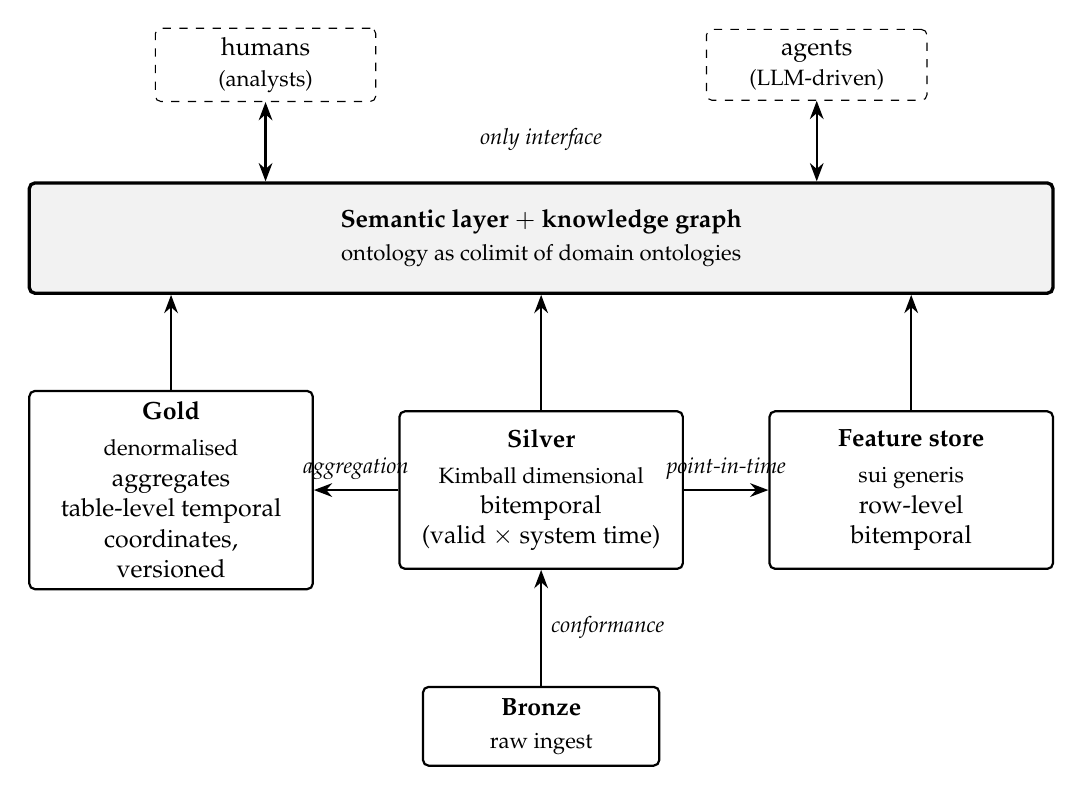
\begin{tikzpicture}[
  every node/.style={font=\small},
  layer/.style={
    rectangle, draw, thick, rounded corners=2pt,
    minimum width=3.6cm, minimum height=2cm,
    align=center, inner sep=4pt
  },
  semantic/.style={
    rectangle, draw, very thick, rounded corners=2pt,
    minimum width=13cm, minimum height=1.4cm,
    align=center, fill=black!5
  },
  consumer/.style={
    rectangle, draw, dashed, rounded corners=2pt,
    minimum width=2.8cm, minimum height=0.9cm,
    align=center
  },
  caption/.style={font=\footnotesize\itshape},
  >=Stealth
]

% ---- Bronze (bottom, beneath silver) ----
\node[layer, minimum width=3cm, minimum height=1cm]
  (bronze) at (0, 0) {\textbf{Bronze}\\[1pt]\footnotesize raw ingest};

% ---- Silver / Gold / Feature Store (middle row) ----
\node[layer] (silver) at (0, 3.0)
  {\textbf{Silver}\\[2pt]\footnotesize
   Kimball dimensional\\
   bitemporal\\
   (valid $\times$ system time)};

\node[layer] (gold) at (-4.7, 3.0)
  {\textbf{Gold}\\[2pt]\footnotesize
   denormalised\\
   aggregates\\
   table-level temporal\\
   coordinates,\\
   versioned};

\node[layer] (feature) at (4.7, 3.0)
  {\textbf{Feature store}\\[2pt]\footnotesize
   sui generis\\
   row-level\\
   bitemporal};

% ---- Semantic layer (above the middle row) ----
\node[semantic] (semantic) at (0, 6.2)
  {\textbf{Semantic layer $+$ knowledge graph}\\[1pt]
   \footnotesize ontology as colimit of domain ontologies};

% ---- Consumers (top) ----
\node[consumer] (humans) at (-3.5, 8.4) {humans\\\footnotesize (analysts)};
\node[consumer] (agents) at (3.5, 8.4) {agents\\\footnotesize (LLM-driven)};

% ---- Arrows: ingestion ----
\draw[->, thick] (bronze) -- node[right, caption, pos=0.5] {conformance} (silver);

% ---- Arrows: silver feeds gold and feature ----
\draw[->, thick] (silver.west) --
  node[above, caption] {aggregation} (gold.east);
\draw[->, thick] (silver.east) --
  node[above, caption] {point-in-time} (feature.west);

% ---- Arrows: each layer up to semantic ----
\draw[->, thick] (silver.north) -- (semantic.south);
\draw[->, thick] (gold.north) -- (semantic.south -| gold.north);
\draw[->, thick] (feature.north) -- (semantic.south -| feature.north);

% ---- Arrows: semantic to consumers (bidirectional) ----
\draw[<->, thick] (semantic.north -| humans.south) -- (humans.south);
\draw[<->, thick] (semantic.north -| agents.south) -- (agents.south);

% ---- "Only interface" label between semantic and consumers ----
\node[caption] at (0, 7.45) {only interface};

\end{tikzpicture}

%     (called from within a figure environment)
%
%   - Standalone compilation: wrap with
%       \documentclass[border=10pt]{standalone}
%       \usepackage{tikz}
%       \usetikzlibrary{positioning, arrows.meta, calc}
%       \begin{document}
%         % ============================================================
% fig_architecture.tex
%
% Hybrid architecture diagram for "Context per Token".
%
% Usage:
%   - Inside the main paper: \input{fig_architecture}
%     (called from within a figure environment)
%
%   - Standalone compilation: wrap with
%       \documentclass[border=10pt]{standalone}
%       \usepackage{tikz}
%       \usetikzlibrary{positioning, arrows.meta, calc}
%       \begin{document}
%         \input{fig_architecture}
%       \end{document}
%
% Requires TikZ libraries: positioning, arrows.meta, calc
% ============================================================

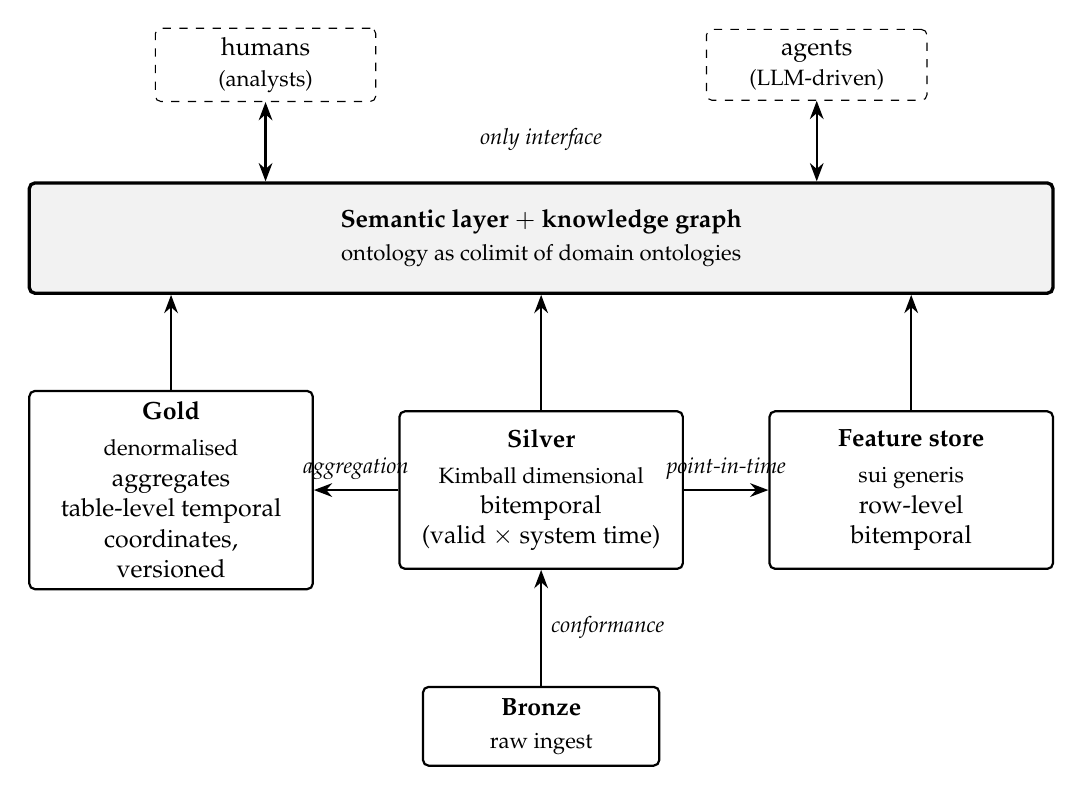
\begin{tikzpicture}[
  every node/.style={font=\small},
  layer/.style={
    rectangle, draw, thick, rounded corners=2pt,
    minimum width=3.6cm, minimum height=2cm,
    align=center, inner sep=4pt
  },
  semantic/.style={
    rectangle, draw, very thick, rounded corners=2pt,
    minimum width=13cm, minimum height=1.4cm,
    align=center, fill=black!5
  },
  consumer/.style={
    rectangle, draw, dashed, rounded corners=2pt,
    minimum width=2.8cm, minimum height=0.9cm,
    align=center
  },
  caption/.style={font=\footnotesize\itshape},
  >=Stealth
]

% ---- Bronze (bottom, beneath silver) ----
\node[layer, minimum width=3cm, minimum height=1cm]
  (bronze) at (0, 0) {\textbf{Bronze}\\[1pt]\footnotesize raw ingest};

% ---- Silver / Gold / Feature Store (middle row) ----
\node[layer] (silver) at (0, 3.0)
  {\textbf{Silver}\\[2pt]\footnotesize
   Kimball dimensional\\
   bitemporal\\
   (valid $\times$ system time)};

\node[layer] (gold) at (-4.7, 3.0)
  {\textbf{Gold}\\[2pt]\footnotesize
   denormalised\\
   aggregates\\
   table-level temporal\\
   coordinates,\\
   versioned};

\node[layer] (feature) at (4.7, 3.0)
  {\textbf{Feature store}\\[2pt]\footnotesize
   sui generis\\
   row-level\\
   bitemporal};

% ---- Semantic layer (above the middle row) ----
\node[semantic] (semantic) at (0, 6.2)
  {\textbf{Semantic layer $+$ knowledge graph}\\[1pt]
   \footnotesize ontology as colimit of domain ontologies};

% ---- Consumers (top) ----
\node[consumer] (humans) at (-3.5, 8.4) {humans\\\footnotesize (analysts)};
\node[consumer] (agents) at (3.5, 8.4) {agents\\\footnotesize (LLM-driven)};

% ---- Arrows: ingestion ----
\draw[->, thick] (bronze) -- node[right, caption, pos=0.5] {conformance} (silver);

% ---- Arrows: silver feeds gold and feature ----
\draw[->, thick] (silver.west) --
  node[above, caption] {aggregation} (gold.east);
\draw[->, thick] (silver.east) --
  node[above, caption] {point-in-time} (feature.west);

% ---- Arrows: each layer up to semantic ----
\draw[->, thick] (silver.north) -- (semantic.south);
\draw[->, thick] (gold.north) -- (semantic.south -| gold.north);
\draw[->, thick] (feature.north) -- (semantic.south -| feature.north);

% ---- Arrows: semantic to consumers (bidirectional) ----
\draw[<->, thick] (semantic.north -| humans.south) -- (humans.south);
\draw[<->, thick] (semantic.north -| agents.south) -- (agents.south);

% ---- "Only interface" label between semantic and consumers ----
\node[caption] at (0, 7.45) {only interface};

\end{tikzpicture}

%       \end{document}
%
% Requires TikZ libraries: positioning, arrows.meta, calc
% ============================================================

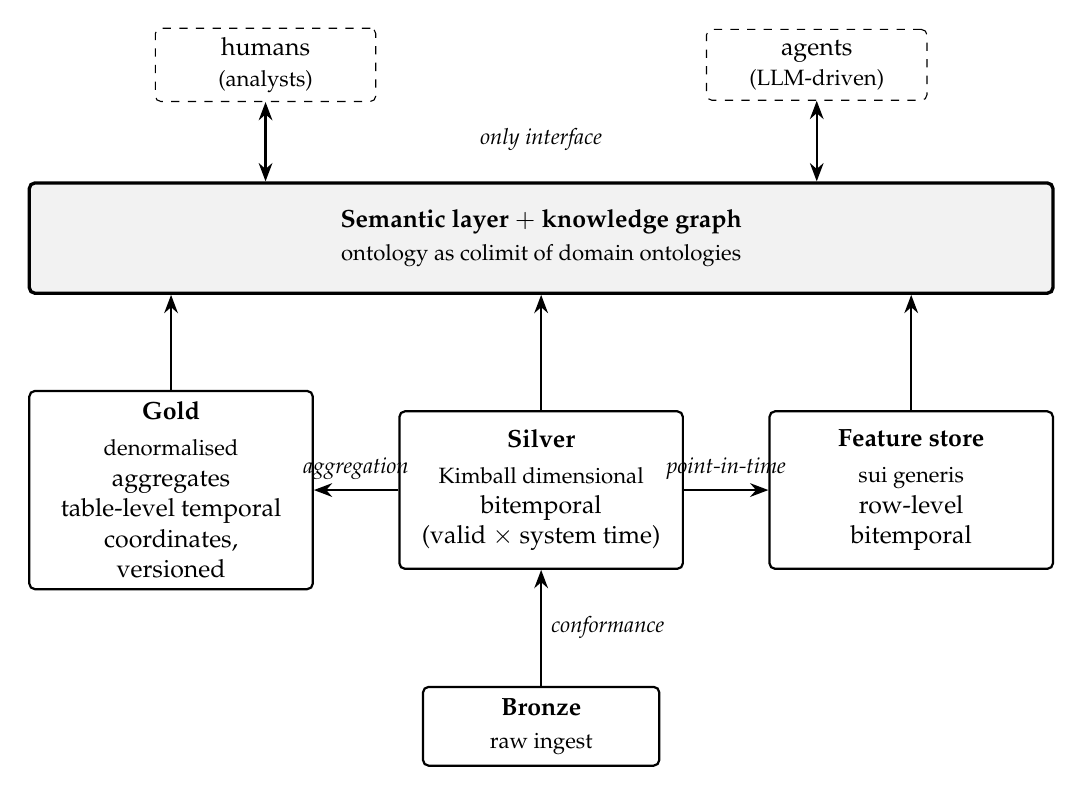
\begin{tikzpicture}[
  every node/.style={font=\small},
  layer/.style={
    rectangle, draw, thick, rounded corners=2pt,
    minimum width=3.6cm, minimum height=2cm,
    align=center, inner sep=4pt
  },
  semantic/.style={
    rectangle, draw, very thick, rounded corners=2pt,
    minimum width=13cm, minimum height=1.4cm,
    align=center, fill=black!5
  },
  consumer/.style={
    rectangle, draw, dashed, rounded corners=2pt,
    minimum width=2.8cm, minimum height=0.9cm,
    align=center
  },
  caption/.style={font=\footnotesize\itshape},
  >=Stealth
]

% ---- Bronze (bottom, beneath silver) ----
\node[layer, minimum width=3cm, minimum height=1cm]
  (bronze) at (0, 0) {\textbf{Bronze}\\[1pt]\footnotesize raw ingest};

% ---- Silver / Gold / Feature Store (middle row) ----
\node[layer] (silver) at (0, 3.0)
  {\textbf{Silver}\\[2pt]\footnotesize
   Kimball dimensional\\
   bitemporal\\
   (valid $\times$ system time)};

\node[layer] (gold) at (-4.7, 3.0)
  {\textbf{Gold}\\[2pt]\footnotesize
   denormalised\\
   aggregates\\
   table-level temporal\\
   coordinates,\\
   versioned};

\node[layer] (feature) at (4.7, 3.0)
  {\textbf{Feature store}\\[2pt]\footnotesize
   sui generis\\
   row-level\\
   bitemporal};

% ---- Semantic layer (above the middle row) ----
\node[semantic] (semantic) at (0, 6.2)
  {\textbf{Semantic layer $+$ knowledge graph}\\[1pt]
   \footnotesize ontology as colimit of domain ontologies};

% ---- Consumers (top) ----
\node[consumer] (humans) at (-3.5, 8.4) {humans\\\footnotesize (analysts)};
\node[consumer] (agents) at (3.5, 8.4) {agents\\\footnotesize (LLM-driven)};

% ---- Arrows: ingestion ----
\draw[->, thick] (bronze) -- node[right, caption, pos=0.5] {conformance} (silver);

% ---- Arrows: silver feeds gold and feature ----
\draw[->, thick] (silver.west) --
  node[above, caption] {aggregation} (gold.east);
\draw[->, thick] (silver.east) --
  node[above, caption] {point-in-time} (feature.west);

% ---- Arrows: each layer up to semantic ----
\draw[->, thick] (silver.north) -- (semantic.south);
\draw[->, thick] (gold.north) -- (semantic.south -| gold.north);
\draw[->, thick] (feature.north) -- (semantic.south -| feature.north);

% ---- Arrows: semantic to consumers (bidirectional) ----
\draw[<->, thick] (semantic.north -| humans.south) -- (humans.south);
\draw[<->, thick] (semantic.north -| agents.south) -- (agents.south);

% ---- "Only interface" label between semantic and consumers ----
\node[caption] at (0, 7.45) {only interface};

\end{tikzpicture}

%     (called from within a figure environment)
%
%   - Standalone compilation: wrap with
%       \documentclass[border=10pt]{standalone}
%       \usepackage{tikz}
%       \usetikzlibrary{positioning, arrows.meta, calc}
%       \begin{document}
%         % ============================================================
% fig_architecture.tex
%
% Hybrid architecture diagram for "Context per Token".
%
% Usage:
%   - Inside the main paper: % ============================================================
% fig_architecture.tex
%
% Hybrid architecture diagram for "Context per Token".
%
% Usage:
%   - Inside the main paper: \input{fig_architecture}
%     (called from within a figure environment)
%
%   - Standalone compilation: wrap with
%       \documentclass[border=10pt]{standalone}
%       \usepackage{tikz}
%       \usetikzlibrary{positioning, arrows.meta, calc}
%       \begin{document}
%         \input{fig_architecture}
%       \end{document}
%
% Requires TikZ libraries: positioning, arrows.meta, calc
% ============================================================

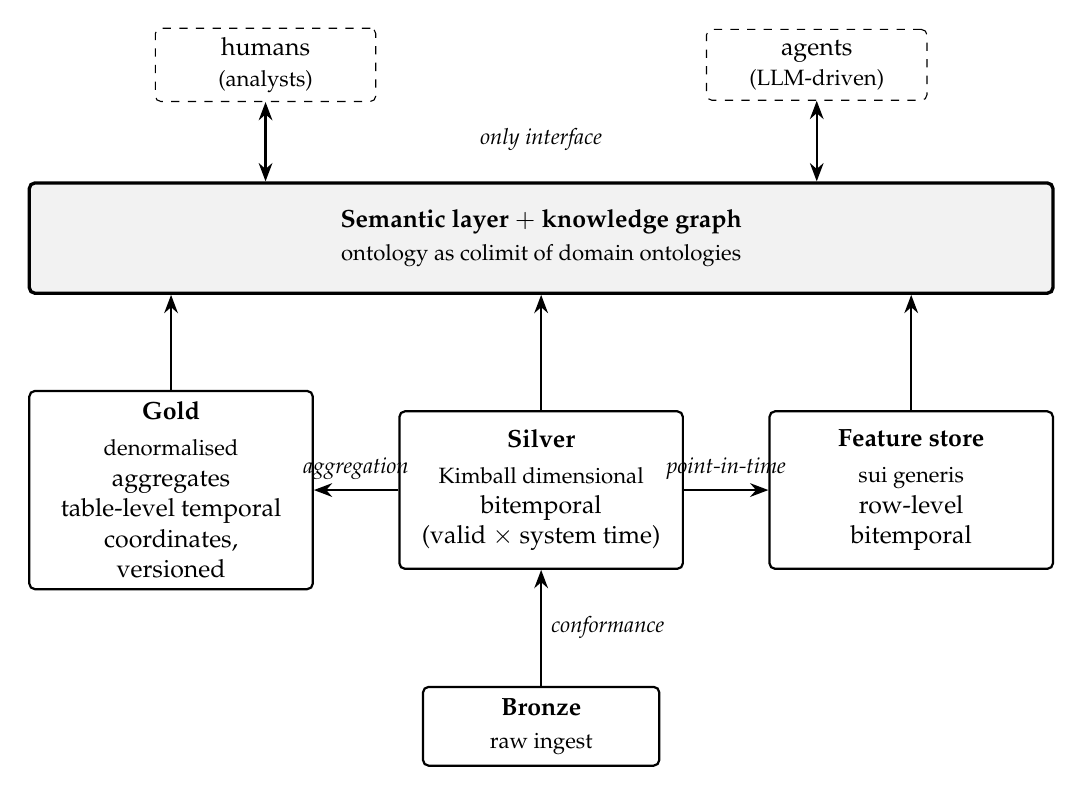
\begin{tikzpicture}[
  every node/.style={font=\small},
  layer/.style={
    rectangle, draw, thick, rounded corners=2pt,
    minimum width=3.6cm, minimum height=2cm,
    align=center, inner sep=4pt
  },
  semantic/.style={
    rectangle, draw, very thick, rounded corners=2pt,
    minimum width=13cm, minimum height=1.4cm,
    align=center, fill=black!5
  },
  consumer/.style={
    rectangle, draw, dashed, rounded corners=2pt,
    minimum width=2.8cm, minimum height=0.9cm,
    align=center
  },
  caption/.style={font=\footnotesize\itshape},
  >=Stealth
]

% ---- Bronze (bottom, beneath silver) ----
\node[layer, minimum width=3cm, minimum height=1cm]
  (bronze) at (0, 0) {\textbf{Bronze}\\[1pt]\footnotesize raw ingest};

% ---- Silver / Gold / Feature Store (middle row) ----
\node[layer] (silver) at (0, 3.0)
  {\textbf{Silver}\\[2pt]\footnotesize
   Kimball dimensional\\
   bitemporal\\
   (valid $\times$ system time)};

\node[layer] (gold) at (-4.7, 3.0)
  {\textbf{Gold}\\[2pt]\footnotesize
   denormalised\\
   aggregates\\
   table-level temporal\\
   coordinates,\\
   versioned};

\node[layer] (feature) at (4.7, 3.0)
  {\textbf{Feature store}\\[2pt]\footnotesize
   sui generis\\
   row-level\\
   bitemporal};

% ---- Semantic layer (above the middle row) ----
\node[semantic] (semantic) at (0, 6.2)
  {\textbf{Semantic layer $+$ knowledge graph}\\[1pt]
   \footnotesize ontology as colimit of domain ontologies};

% ---- Consumers (top) ----
\node[consumer] (humans) at (-3.5, 8.4) {humans\\\footnotesize (analysts)};
\node[consumer] (agents) at (3.5, 8.4) {agents\\\footnotesize (LLM-driven)};

% ---- Arrows: ingestion ----
\draw[->, thick] (bronze) -- node[right, caption, pos=0.5] {conformance} (silver);

% ---- Arrows: silver feeds gold and feature ----
\draw[->, thick] (silver.west) --
  node[above, caption] {aggregation} (gold.east);
\draw[->, thick] (silver.east) --
  node[above, caption] {point-in-time} (feature.west);

% ---- Arrows: each layer up to semantic ----
\draw[->, thick] (silver.north) -- (semantic.south);
\draw[->, thick] (gold.north) -- (semantic.south -| gold.north);
\draw[->, thick] (feature.north) -- (semantic.south -| feature.north);

% ---- Arrows: semantic to consumers (bidirectional) ----
\draw[<->, thick] (semantic.north -| humans.south) -- (humans.south);
\draw[<->, thick] (semantic.north -| agents.south) -- (agents.south);

% ---- "Only interface" label between semantic and consumers ----
\node[caption] at (0, 7.45) {only interface};

\end{tikzpicture}

%     (called from within a figure environment)
%
%   - Standalone compilation: wrap with
%       \documentclass[border=10pt]{standalone}
%       \usepackage{tikz}
%       \usetikzlibrary{positioning, arrows.meta, calc}
%       \begin{document}
%         % ============================================================
% fig_architecture.tex
%
% Hybrid architecture diagram for "Context per Token".
%
% Usage:
%   - Inside the main paper: \input{fig_architecture}
%     (called from within a figure environment)
%
%   - Standalone compilation: wrap with
%       \documentclass[border=10pt]{standalone}
%       \usepackage{tikz}
%       \usetikzlibrary{positioning, arrows.meta, calc}
%       \begin{document}
%         \input{fig_architecture}
%       \end{document}
%
% Requires TikZ libraries: positioning, arrows.meta, calc
% ============================================================

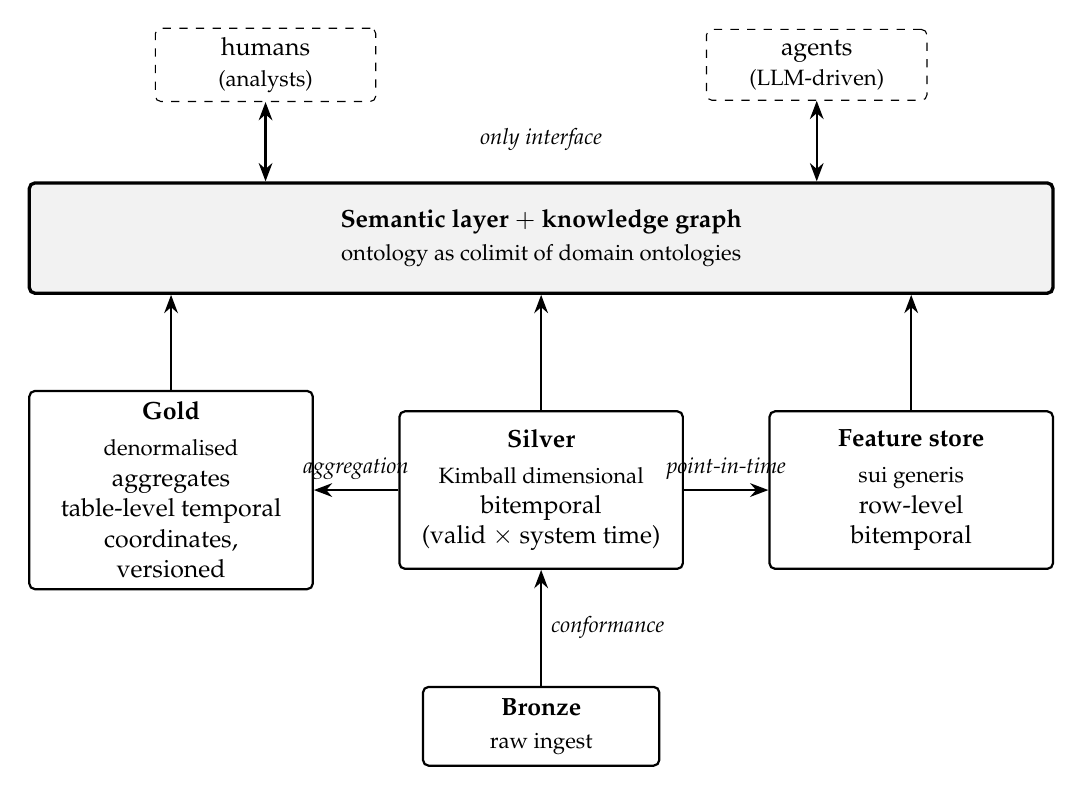
\begin{tikzpicture}[
  every node/.style={font=\small},
  layer/.style={
    rectangle, draw, thick, rounded corners=2pt,
    minimum width=3.6cm, minimum height=2cm,
    align=center, inner sep=4pt
  },
  semantic/.style={
    rectangle, draw, very thick, rounded corners=2pt,
    minimum width=13cm, minimum height=1.4cm,
    align=center, fill=black!5
  },
  consumer/.style={
    rectangle, draw, dashed, rounded corners=2pt,
    minimum width=2.8cm, minimum height=0.9cm,
    align=center
  },
  caption/.style={font=\footnotesize\itshape},
  >=Stealth
]

% ---- Bronze (bottom, beneath silver) ----
\node[layer, minimum width=3cm, minimum height=1cm]
  (bronze) at (0, 0) {\textbf{Bronze}\\[1pt]\footnotesize raw ingest};

% ---- Silver / Gold / Feature Store (middle row) ----
\node[layer] (silver) at (0, 3.0)
  {\textbf{Silver}\\[2pt]\footnotesize
   Kimball dimensional\\
   bitemporal\\
   (valid $\times$ system time)};

\node[layer] (gold) at (-4.7, 3.0)
  {\textbf{Gold}\\[2pt]\footnotesize
   denormalised\\
   aggregates\\
   table-level temporal\\
   coordinates,\\
   versioned};

\node[layer] (feature) at (4.7, 3.0)
  {\textbf{Feature store}\\[2pt]\footnotesize
   sui generis\\
   row-level\\
   bitemporal};

% ---- Semantic layer (above the middle row) ----
\node[semantic] (semantic) at (0, 6.2)
  {\textbf{Semantic layer $+$ knowledge graph}\\[1pt]
   \footnotesize ontology as colimit of domain ontologies};

% ---- Consumers (top) ----
\node[consumer] (humans) at (-3.5, 8.4) {humans\\\footnotesize (analysts)};
\node[consumer] (agents) at (3.5, 8.4) {agents\\\footnotesize (LLM-driven)};

% ---- Arrows: ingestion ----
\draw[->, thick] (bronze) -- node[right, caption, pos=0.5] {conformance} (silver);

% ---- Arrows: silver feeds gold and feature ----
\draw[->, thick] (silver.west) --
  node[above, caption] {aggregation} (gold.east);
\draw[->, thick] (silver.east) --
  node[above, caption] {point-in-time} (feature.west);

% ---- Arrows: each layer up to semantic ----
\draw[->, thick] (silver.north) -- (semantic.south);
\draw[->, thick] (gold.north) -- (semantic.south -| gold.north);
\draw[->, thick] (feature.north) -- (semantic.south -| feature.north);

% ---- Arrows: semantic to consumers (bidirectional) ----
\draw[<->, thick] (semantic.north -| humans.south) -- (humans.south);
\draw[<->, thick] (semantic.north -| agents.south) -- (agents.south);

% ---- "Only interface" label between semantic and consumers ----
\node[caption] at (0, 7.45) {only interface};

\end{tikzpicture}

%       \end{document}
%
% Requires TikZ libraries: positioning, arrows.meta, calc
% ============================================================

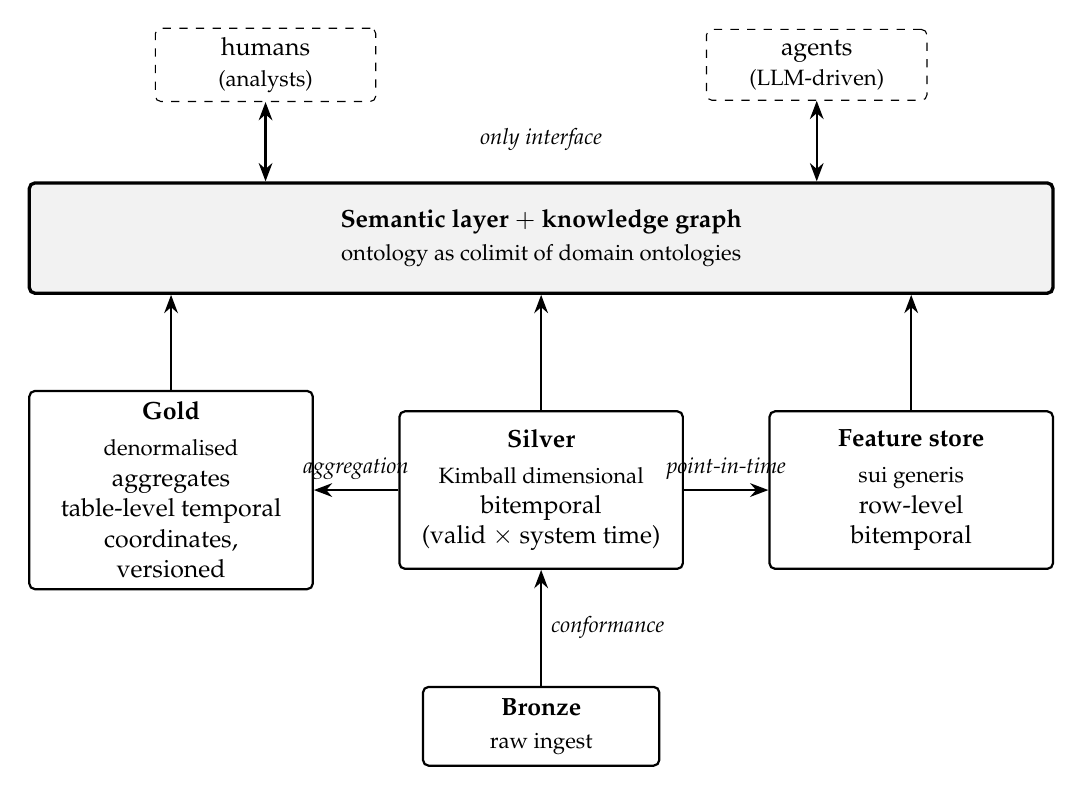
\begin{tikzpicture}[
  every node/.style={font=\small},
  layer/.style={
    rectangle, draw, thick, rounded corners=2pt,
    minimum width=3.6cm, minimum height=2cm,
    align=center, inner sep=4pt
  },
  semantic/.style={
    rectangle, draw, very thick, rounded corners=2pt,
    minimum width=13cm, minimum height=1.4cm,
    align=center, fill=black!5
  },
  consumer/.style={
    rectangle, draw, dashed, rounded corners=2pt,
    minimum width=2.8cm, minimum height=0.9cm,
    align=center
  },
  caption/.style={font=\footnotesize\itshape},
  >=Stealth
]

% ---- Bronze (bottom, beneath silver) ----
\node[layer, minimum width=3cm, minimum height=1cm]
  (bronze) at (0, 0) {\textbf{Bronze}\\[1pt]\footnotesize raw ingest};

% ---- Silver / Gold / Feature Store (middle row) ----
\node[layer] (silver) at (0, 3.0)
  {\textbf{Silver}\\[2pt]\footnotesize
   Kimball dimensional\\
   bitemporal\\
   (valid $\times$ system time)};

\node[layer] (gold) at (-4.7, 3.0)
  {\textbf{Gold}\\[2pt]\footnotesize
   denormalised\\
   aggregates\\
   table-level temporal\\
   coordinates,\\
   versioned};

\node[layer] (feature) at (4.7, 3.0)
  {\textbf{Feature store}\\[2pt]\footnotesize
   sui generis\\
   row-level\\
   bitemporal};

% ---- Semantic layer (above the middle row) ----
\node[semantic] (semantic) at (0, 6.2)
  {\textbf{Semantic layer $+$ knowledge graph}\\[1pt]
   \footnotesize ontology as colimit of domain ontologies};

% ---- Consumers (top) ----
\node[consumer] (humans) at (-3.5, 8.4) {humans\\\footnotesize (analysts)};
\node[consumer] (agents) at (3.5, 8.4) {agents\\\footnotesize (LLM-driven)};

% ---- Arrows: ingestion ----
\draw[->, thick] (bronze) -- node[right, caption, pos=0.5] {conformance} (silver);

% ---- Arrows: silver feeds gold and feature ----
\draw[->, thick] (silver.west) --
  node[above, caption] {aggregation} (gold.east);
\draw[->, thick] (silver.east) --
  node[above, caption] {point-in-time} (feature.west);

% ---- Arrows: each layer up to semantic ----
\draw[->, thick] (silver.north) -- (semantic.south);
\draw[->, thick] (gold.north) -- (semantic.south -| gold.north);
\draw[->, thick] (feature.north) -- (semantic.south -| feature.north);

% ---- Arrows: semantic to consumers (bidirectional) ----
\draw[<->, thick] (semantic.north -| humans.south) -- (humans.south);
\draw[<->, thick] (semantic.north -| agents.south) -- (agents.south);

% ---- "Only interface" label between semantic and consumers ----
\node[caption] at (0, 7.45) {only interface};

\end{tikzpicture}

%       \end{document}
%
% Requires TikZ libraries: positioning, arrows.meta, calc
% ============================================================

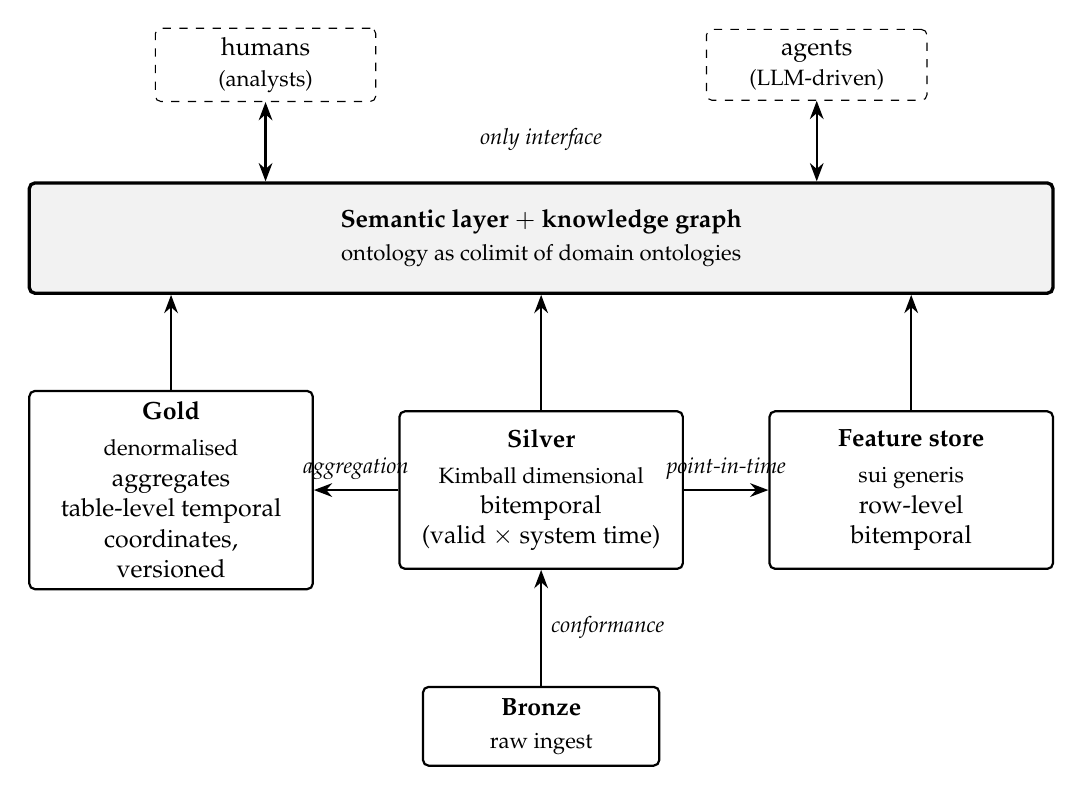
\begin{tikzpicture}[
  every node/.style={font=\small},
  layer/.style={
    rectangle, draw, thick, rounded corners=2pt,
    minimum width=3.6cm, minimum height=2cm,
    align=center, inner sep=4pt
  },
  semantic/.style={
    rectangle, draw, very thick, rounded corners=2pt,
    minimum width=13cm, minimum height=1.4cm,
    align=center, fill=black!5
  },
  consumer/.style={
    rectangle, draw, dashed, rounded corners=2pt,
    minimum width=2.8cm, minimum height=0.9cm,
    align=center
  },
  caption/.style={font=\footnotesize\itshape},
  >=Stealth
]

% ---- Bronze (bottom, beneath silver) ----
\node[layer, minimum width=3cm, minimum height=1cm]
  (bronze) at (0, 0) {\textbf{Bronze}\\[1pt]\footnotesize raw ingest};

% ---- Silver / Gold / Feature Store (middle row) ----
\node[layer] (silver) at (0, 3.0)
  {\textbf{Silver}\\[2pt]\footnotesize
   Kimball dimensional\\
   bitemporal\\
   (valid $\times$ system time)};

\node[layer] (gold) at (-4.7, 3.0)
  {\textbf{Gold}\\[2pt]\footnotesize
   denormalised\\
   aggregates\\
   table-level temporal\\
   coordinates,\\
   versioned};

\node[layer] (feature) at (4.7, 3.0)
  {\textbf{Feature store}\\[2pt]\footnotesize
   sui generis\\
   row-level\\
   bitemporal};

% ---- Semantic layer (above the middle row) ----
\node[semantic] (semantic) at (0, 6.2)
  {\textbf{Semantic layer $+$ knowledge graph}\\[1pt]
   \footnotesize ontology as colimit of domain ontologies};

% ---- Consumers (top) ----
\node[consumer] (humans) at (-3.5, 8.4) {humans\\\footnotesize (analysts)};
\node[consumer] (agents) at (3.5, 8.4) {agents\\\footnotesize (LLM-driven)};

% ---- Arrows: ingestion ----
\draw[->, thick] (bronze) -- node[right, caption, pos=0.5] {conformance} (silver);

% ---- Arrows: silver feeds gold and feature ----
\draw[->, thick] (silver.west) --
  node[above, caption] {aggregation} (gold.east);
\draw[->, thick] (silver.east) --
  node[above, caption] {point-in-time} (feature.west);

% ---- Arrows: each layer up to semantic ----
\draw[->, thick] (silver.north) -- (semantic.south);
\draw[->, thick] (gold.north) -- (semantic.south -| gold.north);
\draw[->, thick] (feature.north) -- (semantic.south -| feature.north);

% ---- Arrows: semantic to consumers (bidirectional) ----
\draw[<->, thick] (semantic.north -| humans.south) -- (humans.south);
\draw[<->, thick] (semantic.north -| agents.south) -- (agents.south);

% ---- "Only interface" label between semantic and consumers ----
\node[caption] at (0, 7.45) {only interface};

\end{tikzpicture}

  \caption{The hybrid architecture. Silver as bitemporal Kimball substrate; gold as denormalised aggregates with table-level temporal coordinates; feature store as sui generis row-level bitemporal layer; semantic layer plus ontology colimit as the sole interface, exposed identically to humans and agents.}
  \label{fig:architecture}
\end{figure}

We treat each substantive layer in turn, naming its purpose, its temporal regime, and what it is not for. Bitemporality is touched lightly here and elaborated in \S\ref{sec:bitemporality}. The ontology colimit is named and elaborated in \S\ref{sec:colimit}. The interface commitment is made structural in \S\ref{sec:interface}.

\subsection{Silver: the bitemporal substrate of truth}

Silver is the substrate. It is built using the dimensional modelling tradition we declined to disavow in \S\ref{sec:pretense} --- grain explicitly chosen and defended per fact table, conformed dimensions across business processes, surrogate keys, SCD2 for tracked attributes. None of this is renegotiated in the agent era. The structural reasons for these patterns have not changed.

What changes is that silver becomes \emph{bitemporal at row level, always}. Every dimension carries both axes --- \texttt{valid\_from}/\texttt{valid\_to} for valid time and \texttt{system\_from}/\texttt{system\_to} for transaction time. Every fact carries an \texttt{event\_timestamp} for what happened in the world and an \texttt{ingestion\_timestamp} plus correction flags for when the warehouse learned about it. An as-of query against silver takes two parameters, not one: as-of valid time, and as-of system time.

This is non-negotiable. The bitemporality of silver is what makes everything downstream auditable, what makes regulatory reconstruction possible, and what makes the silver-versus-gold source-of-truth contract (\S\ref{sec:bitemporality}) coherent. A silver layer that is merely SCD2 --- valid-time only --- fails the moment a correction is applied, because the warehouse cannot then reconstruct what it believed at a prior moment. For an exchange, an investment bank, or any business with regulatory reconstruction obligations, this is unacceptable.

Silver is not denormalised. It does not flatten dimensional attributes into fact rows. It is the compositional substrate over which gold and feature stores are built, and it is also --- directly, when needed --- a queryable layer in its own right, exposed to consumers through the semantic layer with the warning that queries against it pay the join cost.

\subsection{Gold: published denormalisations}

Gold is the publication layer. Its purpose is to answer high-frequency, well-formed questions cheaply, without the join cost of silver and without the latency unpredictability of joining across many dimensions. The pattern is denormalised aggregative views --- wide, flat, materialised, often pre-aggregated at the natural reporting grain: daily P\&L by desk, monthly volume by region, hourly fill rate by venue.

Gold's temporal contract is specific and different from silver's. Gold tables do not carry per-row bitemporal columns. They carry \emph{table-level} temporal coordinates as metadata: an \texttt{as\_of\_valid\_time}, an \texttt{as\_of\_system\_time}, and a \texttt{generated\_at}. The rows are point-in-time materialisations under those coordinates. To audit a gold table, you do not consult per-row history; you re-derive it from silver using the metadata coordinates the table carries.

Gold is therefore \emph{versioned, not mutable}. The right pattern is named versioned tables --- \texttt{gold.pnl\_daily\_v20260520} or its equivalent --- published as immutable artefacts. Each subsequent published version captures the next point in the bitemporal grid. The historical trail is the sequence of versioned tables, with the metadata coordinates serving as the audit index.

This keeps gold's purpose pure: it answers \emph{what was published}, without becoming a second bitemporal substrate competing with silver for source-of-truth status. The contract that governs the silver/gold relationship is treated in \S\ref{sec:bitemporality}; here we note only that the contract becomes coherent precisely because gold does not try to be silver.

A failure mode worth naming. Teams sometimes attempt to make gold ``bitemporal'' by adding row-level valid and system columns, replicating silver's contract one layer up. This collapses the architecture. Two bitemporal substrates means two sources of truth, which means no source of truth, which means audits become arguments. Resist this. Gold's compactness and clarity depend on its temporal contract living at the table level, not the row level.

\subsection{Feature stores: the principled exception}

ML feature stores look like gold but are not. They are a sui generis category in this architecture, and the position requires that they be treated as such.

The defining requirement of a feature store is point-in-time correctness for training data. To train a supervised model honestly, the features available at label-assignment time must be reconstructible exactly --- the feature values \emph{as the system would have known them at that moment}, with no leakage from the future. This is bitemporality at row level, governed by training-time correctness rather than reporting-time auditability.

Feature stores therefore inherit silver's per-row bitemporal discipline, but with different consumers (training loops, online inference) and a different contract (point-in-time correctness, low-latency retrieval). They are not gold and should not be governed as gold. We recommend giving them their own architectural category, their own temporal contract documentation, and their own clearly demarcated surface in the semantic layer.

The reason this matters for the position as a whole: if feature stores are quietly governed as a kind of gold, the gold layer's clean table-level temporal contract is undermined, and the architecture devolves into the bitemporality-everywhere pattern we are arguing against. Naming feature stores separately keeps both contracts clean.

\subsection{The semantic layer and the knowledge graph}

The semantic layer plus knowledge graph is the only interface. It exposes silver, gold, and feature stores through a single declared surface: entities, measures, joins, temporal contracts. The ontology --- the relational structure of what these entities are and how they relate --- is built as a colimit of domain ontologies rather than a unified global model.

We treat the colimit construction in \S\ref{sec:colimit} and the documentation discipline that anchors the semantic layer in \S\ref{sec:documentation}. We treat the only-interface commitment as a structural principle in \S\ref{sec:interface}. Here we name the layer and place it in the architecture.

What matters for the architecture as a whole: every consumer --- human analyst or LLM-driven agent --- enters through this layer. There are no direct paths to silver, to gold, or to feature stores that bypass it. The cost of this commitment is significant; the benefit is that information density per token is governed in one place, that temporal contracts are surfaced uniformly, and that the ontology is the single object that humans and agents reason over. Without this commitment, the architecture is a collection of layers without a common interface. With it, the architecture is one system.

The sections that follow elaborate the parts of this commitment that need defence: bitemporality and the source-of-truth contract (\S\ref{sec:bitemporality}), the colimit construction and the morphism discipline (\S\ref{sec:colimit}), documentation as reasoning-context (\S\ref{sec:documentation}), the only-interface principle (\S\ref{sec:interface}), and what all of this demands of teams in practice (\S\ref{sec:demands}).

% ============================================================
\section{Bitemporality and the Source of Truth}
\label{sec:bitemporality}
% ============================================================

\S\ref{sec:hybrid} stated the temporal regime of each layer. This section makes the regime operational. The architectural problem bitemporality solves is straightforward to state and consistently underdone in practice: at any moment after the present one, somebody --- auditor, regulator, analyst, model --- will ask a question about what happened on a particular date, and the question they ask will be one of two structurally different questions. The architecture must answer both, and must keep them distinguishable.

\subsection{The two questions}

The first question is: \emph{what was true?} --- meaning, what is now known about the state of the world on that date. Late-arriving facts have been received. Corrections have been applied. Reclassifications have been processed. The answer is the warehouse's current best reconstruction of the past, with everything we have learned since.

The second question is: \emph{what was reported?} --- meaning, what did the system say at the time. This is not the same answer. The reports we produced on day $T$ were produced from the data the warehouse held on day $T$, and that data has since been corrected, augmented, and reclassified. The reports are themselves part of the historical record --- what regulators received, what management acted on, what compensation committees used. The number we now believe and the number we then published are both real, both have legitimate uses, and conflating them is how audits become arguments.

A bitemporal architecture exists to keep both answers retrievable, distinguishable, and cheap to obtain. The two questions are the architecture's load.

\subsection{The contract}

The position is one sentence: \emph{gold is authoritative for what was reported; silver is authoritative for what was true; bitemporality reconciles them.}

Silver carries both temporal axes at row level. As of any valid time and any system time, silver can be queried for what the warehouse's best reconstruction of the world was at that moment. Corrections in silver supersede rather than overwrite --- the prior row remains, closed by its \texttt{system\_to} timestamp, and the corrected row appears with its \texttt{system\_from} timestamp set to the moment of correction. Silver's history of beliefs is preserved.

Gold carries table-level temporal coordinates as metadata. Each published gold version is immutable. The published \texttt{gold.pnl\_daily\_v20260520} is exactly what was reported on that date, computed from silver as silver stood at that date. When silver is corrected, gold is not retroactively rewritten. A new gold version is published --- \texttt{gold.pnl\_daily\_v20260603}, say --- capturing the latest understanding. Both versions remain. The audit trail is the sequence.

The semantic layer surfaces this contract directly. Queries against gold receive published-as-of semantics by default; queries against silver receive truth-as-now-known semantics by default; both surfaces accept explicit as-of coordinates when the caller needs to override.

\subsection{Correction events}

A correction is the moment the contract is exercised. Consider what happens, end to end, when an upstream trade-capture system issues a correction to a counterparty assignment for a trade booked three weeks ago.

In silver, the correction arrives as a new row on the execution fact --- same \texttt{event\_timestamp}, new \texttt{cpty\_id}, with \texttt{system\_from} set to the correction's arrival and the prior row's \texttt{system\_to} set to the same moment. The prior row is not deleted. The counterparty dimension may also be touched if the correction's reasoning involves a counterparty record change; in that case the same supersession discipline applies on the dimension.

In gold, the correction does not propagate retroactively. The gold P\&L tables published in the three weeks since the original booking remain as they were published. The next scheduled gold rebuild --- daily, hourly, whatever the cadence --- picks up the corrected silver and produces a new gold version that incorporates it. The published audit trail is now: the original gold versions, plus the post-correction versions, with the correction visible by comparing them.

In the semantic layer, the change surfaces as a temporal metadata update on the relevant gold tables and a silver row supersession in the bitemporal log. An agent that queries ``what is the P\&L for desk $X$ on date $Y$'' through the semantic layer receives the current best reconstruction --- from silver, or from the most recent gold version if gold is the queried surface. An agent that queries ``what was reported for desk $X$ on date $Y$ as of date $T$'' receives the gold version that was current on date $T$. Both queries are first-class. Neither is a default that hides the other.

\subsection{The query vocabulary}

The semantic layer needs three query modes to make the contract usable, and they should be named explicitly rather than left implicit in caller convention.

The first is \emph{as-of-now over current-truth}: silver queried with both axes set to now. This is the default for most analytical work. The second is \emph{as-of-valid-time over current-truth}: silver queried with valid time set to the historical moment of interest and system time set to now. This is the dominant mode for analytical questions about prior states of the world. The third is \emph{as-of-report-time}: gold queried by its version coordinate, or silver queried with system time set to a historical moment. This is the mode that regulators, reconciliation processes, and any consumer asking ``what did we know on the day we reported'' uses.

The \S\ref{sec:binding} example surfaced the first two implicitly: ``tier at execution time'' is as-of-valid-time over current-truth; ``current tier'' is as-of-now over current-truth. The third mode --- what we reported on a prior date --- was outside that question's scope but is the one that audits and reconciliations lean on hardest. All three need to be first-class in the semantic layer's vocabulary, surfaced in the documentation, and reasoned over by agents without ambiguity.

\subsection{Why this matters more than it appears}

The temptation, especially in lakehouse-era teams, is to treat bitemporality as a regulatory tax --- something compliance demands, something the analytics team works around with a sigh. The position of this paper is that this framing is exactly backwards. Bitemporality is not a tax on the analytical substrate. It is what makes the analytical substrate trustworthy when the consumer of the data --- human or agent --- has no other way to verify what it is being told.

An agent reading a gold table with a \texttt{generated\_at} coordinate knows what the answer is conditioned on. An agent querying silver with explicit as-of-valid-time and as-of-system-time parameters knows exactly what it is asking for and what it will receive. The bitemporal discipline turns out to be the most legible context an agentic consumer can receive about temporal claims, precisely because it removes the implicit. There is no tribal knowledge to import. The temporal contract is on the surface.

The same discipline that makes the warehouse defensible in an audit is the discipline that makes it legible to an agent. The regulatory consumer and the agentic consumer converge on the same design --- a coincidence that will repeat through the rest of this paper, and one worth noticing each time it does.

% ============================================================
\section{Ontology as Colimit}
\label{sec:colimit}
% ============================================================

The information-architecture tradition, the data-cataloguing tradition, and the metadata-management tradition have between them spent thirty years trying to build the thing this section will sketch in a paragraph. The teams that own metadata catalogues in large enterprises --- Collibra, Alation, their predecessors, their successors --- have, by and large, terrible reputations across financial services, manufacturing, healthcare, and the public sector. The projects are slow. The models are never finished. The owners are seen as blockers. The reputations are well-earned in the local sense that the work has not delivered. They are unfair in the structural sense that the architectural framework these teams were given is the wrong framework, and inside it the work cannot be finished.

The colimit construction is the right framework. What follows is the case for it, the demonstration that it makes the work finishable, and an honest treatment of the additional axis that has been almost entirely absent from the IA tradition: the bitemporality of meaning itself.

\subsection{Why naive unification fails}

The instinct of every information architect who has ever tried to build an enterprise ontology is unification. One Customer. One Product. One Account. A single global model, owned centrally, against which all downstream systems are eventually conformed. This is the model behind every ``single source of truth'' programme, every master data management initiative, every metadata catalogue rollout that promises to harmonise the enterprise.

It does not work, and the reason is not implementation failure. The reason is that the local domains are not wrong about their definitions. Compliance's Customer is a KYC-segmented legal entity with regulatory classifications, jurisdiction tags, and onboarding lineage. Trading's Customer is a counterparty with a credit limit, a tier, an exposure profile, and a netting agreement. Marketing's Customer is a segmented prospect or account with lifecycle status, channel attribution, and opportunity history. Each of these is correct in its own domain. None of them is reducible to any of the others.

Force them into a unified model and one of two things happens. Either the unified model becomes the union of all local attributes --- at which point it is no longer a model, it is a flat schema with hundreds of columns, half of them irrelevant to any given consumer --- or the unified model is the intersection, the lowest common denominator, which loses the information that makes each local domain useful in the first place. Both outcomes are failure modes. The first is what most enterprise data dictionaries actually become. The second is what most ``core entity'' definitions degrade to. Either way, the central team is held responsible for a deliverable the framework has made impossible.

\subsection{Why naive federation fails}

The opposite instinct, which the data mesh literature has popularised, is federation. Let each domain own its own ontology. Stop trying to unify. Trust the domains to know their own data. Compose downstream by referencing local definitions.

This is closer to right, but it is not the answer alone. Consumers --- and especially agentic consumers --- must traverse across domains to answer real questions. ``Net P\&L by customer segment for European institutional counterparties'' touches trading, compliance, and at least one regional classification scheme. Under pure federation, an agent has access to three local ontologies and no declared way to compose across them. It either invents the compositions, which is hallucination, or it falls back to direct table joins, which is the regression the previous four sections of this paper have been arguing against.

Federation without compatibility maps is silos with extra documentation. The question is not whether to federate. The question is what the compatibility maps look like.

\subsection{The colimit}

A colimit, in the category-theoretic sense, is the construction that glues a collection of local objects together along explicit maps, producing a global object that respects every local object and every map, without forcing the locals into a single uniform shape. Stated for an enterprise data engineering audience: a colimit ontology is the global structure that emerges when each domain ontology is preserved as itself, and the translation maps between domains are written down explicitly. The global object is not a unified model. It is the structure determined by the local models and the maps between them.

This is the right framework for three reasons.

It preserves local truth. Compliance's Customer remains compliance's Customer. Trading's Customer remains trading's Customer. Neither is overwritten or reduced. The work of the central team is not to decide which is correct. The work is to write down honestly how they relate.

It is finishable. The IA tradition's reputation for slow, perpetually-incomplete models is a direct consequence of the unification framework: a unified model is never finished because the domains keep diverging and the central definition keeps having to be renegotiated. A colimit is finished, locally, when a local ontology is captured and the morphisms to its neighbours are written down. The whole is never ``complete'' in a global sense, but no part needs to be globally complete before it is useful.

The morphisms are exactly the structural information that agentic consumers need. An agent traversing from a compliance question to a trading question reads the morphism between Compliance.Customer and Trading.Counterparty and knows how to compose. There is no inference required, no hallucination of relationships. The maps are first-class objects in the architecture.

\subsection{The morphisms are the entire game}

A colimit construction without honest morphisms is unification with extra ceremony. The architectural discipline that turns the colimit from a framework into engineering is morphism honesty.

An honest morphism between two domain entities is an explicit, named, dated, signed piece of documentation that states what the source entity maps to in the target, what attributes survive the map, what attributes are lost in the map, what attributes the target adds that the source does not constrain, where the map is partial on either side, who in each domain signed off, and when it was last reviewed. Each of these is named explicitly. The losses and partialities are named explicitly. Nothing is implicit.

Consider, concretely, the morphism from Compliance.Customer to Trading.Counterparty in a mid-tier investment bank. The map is well-defined for institutional clients onboarded through the compliance KYC process: Compliance.Customer.\texttt{legal\_entity\_id} is the source key, Trading.Counterparty.\texttt{cpty\_id} carries the foreign key, the relationship is one-to-many because a single legal entity may have multiple trading accounts. The map loses Compliance.Customer.\texttt{kyc\_sub\_segment}, which has no Trading.Counterparty counterpart; the trading desk does not require KYC sub-segmentation, and forcing it through would corrupt the trading model with attributes that have no operational meaning on that side. The map is partial on the target side: certain trading counterparties --- proprietary desks, market-making subsidiaries --- do not have a Compliance.Customer antecedent because they are internal entities. The map is signed by the head of compliance data and the head of trading data, and the date of last review is the most recent regulatory inflection point.

This is what every morphism between every pair of domain entities looks like. It is unglamorous work. It is exactly the work the colimit framework requires and the unification framework hides under the carpet.

\subsection{Meaning over time}

The information-architecture tradition has been almost entirely silent on a question that turns out to be load-bearing: ontologies themselves change. Compliance's Customer definition in 2026 is not Compliance's Customer definition in 2024 --- MiCA changed it, materially. The compliance-to-trading morphism in 2026 is not the morphism that held in 2024, because the source object on one side of the map has shifted. An agent reading 2024 compliance documentation against 2026 trading data, with whatever morphism happens to be current, will produce confidently wrong answers about historical states of the world.

The discipline \S\ref{sec:bitemporality} imposed on data --- bitemporality, two-axis as-of queries, audit trails through versioned artefacts --- applies in full to the ontology layer. Each domain ontology is itself a bitemporal object, with a valid time (when the definition applied in the world) and a system time (when it was written down). Each morphism is bitemporal: it has a date of last review and it is keyed against the versions of the source and target ontologies it connects.

A practical consequence: an agent asking a historical question --- ``what was the segment of customer $X$ in Q3 2024'' --- must be served the ontology that was current in Q3 2024, mapped through the morphisms that held then, not the ontology current today. The semantic layer must surface this. The query is bitemporal at the ontology layer as well as the data layer. The two-axis discipline is fractal: it applies wherever meaning is claimed, not just wherever values are stored.

In regulated industries this is the case in nearly every compliance reconstruction, every regulatory inquiry, every restated filing. The reason the IA tradition has been silent on it is that under the unification framework it is unaddressable --- a unified model has one definition, and ``the definition has changed over time'' reduces to ``the model has been wrong at various points,'' which is not a position any central team can defend in front of stakeholders. Under the colimit framework, ontologies and morphisms are versioned, dated, signed objects. Meaning over time becomes a first-class concern rather than an embarrassment.

\subsection{Why this is finishable}

The colimit framework makes the work finishable for a reason that should not be missed: it never requires the whole to be complete in order for the parts to be useful. Each domain ontology can be captured, documented, and served while morphisms to other domains are still being written. Each morphism can be written, signed, and surfaced while other morphisms across the enterprise remain absent. The agent or analyst working in a single domain sees the local ontology immediately. The agent or analyst working across two domains sees the two local ontologies plus the explicit morphism between them. The agent or analyst working across more domains than have been mapped sees the gap, transparently, and can request that the next morphism be written.

This is the operational shape of finishable ontological work. The IA tradition's failure to deliver was not a failure of effort or competence. It was the consequence of working under axioms that made the work intrinsically unfinishable. The colimit framework removes the unfinishability. What remains is unglamorous, disciplined, and unending in the sense that morphisms must be reviewed as ontologies shift over time --- but at every moment the work to date is in production and useful.

The next section makes the case that documentation, in this architecture, is no longer metadata about data but context for reasoning over data, and that the morphisms named in this section are themselves a species of that new documentation object.

% ============================================================
\section{Documentation as Context for Reasoning}
\label{sec:documentation}
% ============================================================

The shift this section describes is the deepest of the paper's commitments, the easiest to overlook, and the one most likely to be resisted by the existing documentation tradition. The shift is this: the consumer of documentation has changed, and the documentation has not changed to match.

For thirty years documentation has been built to be browsed by humans navigating a catalogue and audited by regulators checking that definitions exist. The artefact that resulted --- short, structured, ISO 11179-style controlled-vocabulary entries with name, definition, datatype, permissible values, classification --- was the right artefact for those consumers. It is the wrong artefact for the consumer the agentic era has produced.

\subsection{What ISO 11179 was for}

The controlled-vocabulary tradition, formalised in ISO 11179 and instantiated in every modern data catalogue product, optimised for three things: cross-reference between named entities across systems, schema standardisation as a precondition for integration, and demonstrable compliance with definitional governance. These are real goals. The tradition served them well within its own frame.

What ISO 11179 was never designed for is the transmission of operational knowledge. A short, structured definition tells you the datatype of a column and what the column is called. It does not tell you why the column exists, when its values diverge from the obvious interpretation, what edge cases bite practitioners every quarter, what the desk's slang for it is, how it relates to upstream system quirks, or what a new analyst should know on their second day. All of this is information that exists in the heads of senior practitioners. It is precisely the information the IA tradition has, throughout its history, failed to capture.

This was tolerable when the consumers of data documentation were humans who could absorb operational knowledge by sitting next to senior colleagues for six months. It is not tolerable when the consumer is an LLM agent that has whatever you put in its context and nothing more.

\subsection{The onboarding analogue}

The right way to think about agent-targeted documentation is to think about onboarding a junior analyst.

When you bring a new analyst onto a trading desk or into a treasury function, you do not hand them a metadata catalogue. You hand them prose, and you talk. You tell them the war stories: the time the upstream system reclassified counterparties without warning and broke the morning P\&L for a week. You explain the conventions: how P\&L is computed here, which of the three canonical definitions the desk uses, when it switches to the others. You walk them through the slang: what ``the book'' means in this office, what ``the cross'' means at this desk, which fields are actually used and which are vestigial. You share the craft: how to interpret edge cases, what a sudden gap in a time series typically means, which exceptions are noise and which are signal.

A practical observation, worth pausing on. A capable LLM brings substantial general knowledge to any business domain --- accounting principles, market mechanics, regulatory shape, the standard patterns of analytical work in finance. On day one, that general knowledge frequently exceeds what a junior human analyst arrives with. What it lacks is what the human analyst will spend the next month acquiring: organisational nuance, desk-specific convention, tribal slang, the operational craft of how this particular team uses these particular data assets. After about a month, the human has absorbed enough of that context to function. Without the same context delivered explicitly, the agent never does. It plateaus at general competence, perpetually missing the specifics that distinguish a good analyst from a textbook one.

The documentation that closes this gap looks like onboarding material. It does not look like ISO 11179.

\subsection{The domain essay}

A domain essay, for a single dataset or a tightly coupled cluster of them, is six hundred to fifteen hundred words of considered prose covering provenance, conventions, edge cases, slang, history, and craft. It is written by the people who know the data --- not generated from the schema, which by construction cannot tell you what the schema fails to capture. It is anchored on structured metadata that does not disappear: datatypes, primary keys, refresh cadence, lineage references, ownership records. These anchors are not the documentation. They are the index into it.

The morphisms named in \S\ref{sec:colimit} are themselves a species of essay, focused on the relationship between two domains rather than the substance of one. A compliance-to-trading morphism written as a controlled-vocabulary entry would be the field mapping and nothing else. Written as an essay, it is the field mapping plus the explanation of why KYC sub-segments do not survive the map, why proprietary desks have no compliance antecedent, when the map was last challenged by a regulator, and how the morphism is expected to shift if the next regulatory inflection arrives. This is the format an agent can reason over. It is also the format that lets a new compliance analyst understand how their work touches trading.

\subsection{What this is not}

A few clarifications, because the position invites a particular set of misreadings.

This is not the death of structured metadata. The anchors --- datatype, key, refresh cadence, lineage, ownership --- remain essential. They are machine-readable, automatable, suitable for the cross-reference and integration purposes ISO 11179 was actually good at. The shift is in where the semantic weight lives: from controlled-vocabulary entries as the primary carrier to essays as the primary carrier, with structured metadata as the index.

It is not chatty documentation, or unprofessional documentation, or documentation produced to a lower standard. The right comparison is the operational note a senior practitioner writes for a new colleague: dense, deliberate, evidence-based, free of padding. It happens to be in prose rather than in CV form. That is not a lowering of standards. It is a different format for a different consumer.

Essays are not infinitely long. They are bounded by their subject. Most datasets earn somewhere between six hundred and fifteen hundred words. The rare critical asset --- a primary fact table, a heavily contested dimension --- might earn more. The work is finite. The IA-tradition fear that ``you can't have everyone write essays for everything'' misunderstands the scope; the work is the same total volume the catalogue tradition aspired to, in a denser and more useful form.

Essays are not generated by an LLM from a schema. The whole point is that the essay carries information the schema does not. A schema-generated essay is, by construction, no better than the schema. Essays are written by the people who hold the operational knowledge. LLMs can help draft and edit, but the source of the knowledge is human and organisational.

\subsection{Living, citable, version-controlled}

The discipline that makes essay-based documentation work is the discipline of code. Essays are versioned. They have dated revisions. They have named authors and reviewers. They are stored alongside the data assets they describe and referenced by structured metadata. They have a decay model: an essay reviewed within the last twelve months is treated differently by the semantic layer from one untouched for three years.

This matters because stale documentation is, for an agent, strictly worse than absent documentation. The agent reads stale prose with the same confidence as fresh prose and produces confidently wrong answers. A documentation system that does not manage decay is a documentation system that produces worse outcomes the longer it operates. Version control, dated revisions, and surfacing of staleness through the semantic layer are not optional refinements. They are what makes the architecture safe.

\subsection{The convergence}

A pattern from \S\ref{sec:bitemporality} repeats here. The documentation that lets an agent reason over the data is the documentation that onboards a new human analyst fastest. The same artefact serves the regulator's ``what is this column'' question better than ISO 11179 ever did, because the essay contains the definition plus the operational context that makes the definition usable. The agentic consumer, the new human consumer, and the regulatory consumer converge on the same documentation discipline.

That convergence is the recurring signature of this paper. The agent is not a special consumer with exotic requirements. The agent is the consumer that cannot import tribal knowledge silently, and that inability surfaces what was always wrong with documentation built for browsing rather than reasoning. Build documentation for agents and it gets better for humans. Build it for cataloguing and it has never been good enough for either.

% ============================================================
\section{The Semantic Layer Is the Only Interface}
\label{sec:interface}
% ============================================================

The commitment of this section is the operationally hardest in the paper. Every other commitment lives inside its layer and can be defended on its own terms. This one cuts across the architecture and constrains how every consumer reaches it. It is the commitment that makes the architecture a system rather than a collection of techniques.

The position is: the semantic layer is the only interface between data and consumer, where consumer means human analyst, LLM-driven agent, BI tool, or any other reader of the system. There is no direct SQL access to silver. There is no direct SQL access to gold. There is no analyst's notebook reading parquet files. There is no privileged tier of ``power users'' who get to bypass the semantic layer because they are senior enough to be trusted. The semantic layer is the surface. Everything else is implementation.

\subsection{Why the commitment is structural, not stylistic}

The argument is straightforward. Every other commitment in this architecture is delivered through the semantic layer or through nothing.

Bitemporal contracts (\S\ref{sec:bitemporality}) are surfaced through the semantic layer's declared as-of query modes. A consumer who reaches direct SQL bypasses the contract and conflates the two structurally distinct questions \S\ref{sec:bitemporality} was built to keep separate. They will get plausible answers. They will not know which question they have asked. The contract is the layer's contract, not the database's contract. Without the layer, there is no contract.

The colimit ontology (\S\ref{sec:colimit}) is surfaced through the semantic layer's exposed entities, joins, and morphisms. A consumer who joins silver tables directly bypasses the morphisms entirely, composes by physical key, and reinvents --- badly, locally, inconsistently --- the maps the colimit framework was built to make explicit. After ten such ad-hoc joins, the enterprise has ten incompatible local re-implementations of the same morphism, each with different lossiness, none signed. The colimit dissolves into the silos the IA tradition spent thirty years failing to escape.

Documentation as reasoning-context (\S\ref{sec:documentation}) is surfaced through the semantic layer's exposure of essays, anchors, and decay metadata to its consumers. A consumer who queries direct SQL has access to column names and not much else. They are reasoning over the worst possible representation of the data, the one \S\ref{sec:documentation} was written to argue against. The essay is the layer's surface; the underlying database has no essay.

Information density per token (\S\ref{sec:binding}) is a property of the semantic layer's exposed surface, computed at the moment of consumption. The schema-dump-with-samples failure mode is what happens whenever the semantic layer is bypassed. Every direct-SQL query is, in effect, a low-density context the consumer has chosen for themselves.

These commitments are not separable. They are delivered together through one surface or they are delivered through none.

\subsection{The agentic case}

For LLM-driven agents the only-interface commitment is not a preference. It is a precondition.

An agent reasons over the context it is given. It has no ability to import tribal knowledge from outside that context. The semantic layer's declared surface --- entities, measures, joins, temporal contracts, morphisms, essays, anchors --- is the entire reasoning surface available to the agent. The completeness of the semantic layer is the completeness of the agent's reasoning. There is no second source.

This has a sharp operational consequence. When an agent cannot answer a question through the semantic layer, the response is to extend the semantic layer, not to grant the agent SQL access. Granting SQL access does not solve the problem. It moves it: the agent now reads a low-density context and produces plausible-but-wrong answers with confidence, which is the failure mode of \S\ref{sec:binding} in \S\ref{sec:binding}'s exact form. The agent does not get smarter when given direct access to the underlying tables. It gets more confident about the wrong things.

The structural commitment for agentic consumers is therefore: every gap an agent surfaces is a gap in the semantic layer, not a case for direct access. The remediation is documentation, ontology, morphism, or measure work --- never a bypass.

\subsection{The human case and the direct-SQL anti-pattern}

The harder case is the human one, because the request to bypass the semantic layer is reasonable on its face. A senior analyst needs a number quickly. The semantic layer does not have the slice they need. SQL would take them ten minutes. Why should they wait for an intake ticket?

The answer is uncomfortable. Every such bypass fragments the metric definitions, the temporal contracts, and the ontology morphisms. The number the senior analyst produces in ten minutes is by construction not the number the semantic layer would produce, because they have made the choices the semantic layer makes explicit and they have made them silently. Now there are two definitions of the metric in circulation --- the layer's, and the analyst's notebook's. The layer's is documented. The analyst's is not. Six months later, a junior colleague trying to reproduce the analyst's number cannot, because the analyst has left and their notebook lived on a laptop. The metric is now both authoritative-via-the-layer and authoritative-via-tribal-memory, and the tribal memory has expired.

This is the failure mode the only-interface commitment is built to prevent. It is not theoretical. It is the dominant failure mode of every data programme that grants ``power user'' SQL access for productivity reasons.

The position is therefore: there are no power users. There is the semantic layer. The semantic layer must be fast enough, complete enough, and extensible enough that bypassing it does not feel necessary. When it does feel necessary, the response is to extend the layer, not to grant the bypass. This is unpopular in the short term. It is correct, and worth being unpopular about, because the alternative is the slow fragmentation of every architectural commitment the paper has made.

\subsection{What the semantic layer must do to earn this status}

The commitment runs in both directions. If the semantic layer is the only interface, it must be a serious interface. The obligations on it are correspondingly heavy.

It must be \emph{complete enough for the work}. A semantic layer that exposes ten dashboards' worth of canned measures and stops there is not an interface; it is a reporting surface. The semantic layer must expose every entity, every defensible measure, every meaningful join, every temporal contract, every morphism --- not as a final state but as a continuously expanding surface where the question ``is $X$ available?'' has a near-universal ``yes'' answer for the questions the business actually asks.

It must be \emph{fast enough}. If a query that takes ten seconds through direct SQL takes five minutes through the semantic layer, the layer will be bypassed regardless of governance. Performance is not a nice-to-have. It is the operational precondition for the only-interface commitment to be honoured.

It must be \emph{capable enough for exploratory work}. The most common reason analysts want SQL is that they are exploring --- composing a question they have not asked before, iterating on ideas, sometimes failing and discarding. The semantic layer must support this mode, not only the canned-question mode. If it does not, it has implicitly defined exploration as something that happens outside the architecture, and exploration is exactly where new metric definitions are born and where fragmentation begins.

It must have a \emph{real extension process}. ``Add it to the semantic layer'' must be an intake that returns in days, not quarters. If extending the layer takes longer than building a workaround, the workarounds will accumulate and the layer will atrophy. A semantic-layer team without a working intake is a bottleneck dressed up as governance.

It must be \emph{well-instrumented}. The gaps where consumers reach for bypasses --- agentic or human --- must be visible to the team that owns the layer. Every request the layer cannot serve is signal. Every workaround that emerges in the wild is signal. The layer's owners must see this signal in something closer to real time than a quarterly review.

These obligations are non-trivial. The only-interface commitment is not free. The architectural payoff --- every other commitment in this paper actually delivered to consumers, rather than leaked away through bypasses --- is what justifies the cost.

\subsection{The narrow exceptions}

There are legitimate cases for direct database access below the semantic layer. Honesty requires naming them.

Debugging the data substrate itself --- investigating a data-quality incident, tracing a pipeline failure, reconciling a discrepancy that the semantic layer cannot itself diagnose --- requires direct access. The data engineering team that maintains silver, gold, and the semantic layer needs this access as a matter of their own work on the architecture.

Performance investigation --- understanding why a particular query is slow, examining physical plans, profiling materialisation cost --- requires access below the semantic layer.

Some specialised ML feature engineering, particularly during the early exploration of a new feature space before the feature has been promoted to the feature store, may require direct work against silver. The honest framing is that this is feature engineers operating below the semantic layer, on data that has not yet been declared as a feature in the architecture's terms.

The pattern across these exceptions: they are operations by the people who build the architecture, on the substrate they are responsible for, in service of work that will eventually surface through the semantic layer. They are not consumer queries. They are not ``I need a number for the meeting in an hour.'' They do not produce metrics that enter circulation. They are bounded, governed, logged, and they do not set precedent for routine use.

The discipline is to name these exceptions explicitly and to refuse to let them widen. The data engineering team's debugging access does not become the analytics team's SQL access by drift. The feature engineer's early-exploration window does not become a permanent workaround for any analytical question the semantic layer does not yet serve. Exceptions stay exceptions because they are named, scoped, and reviewed. The moment they are unnamed, the only-interface commitment is dead.

\subsection{The convergence}

The pattern that has run through this paper reasserts itself with particular clarity in this section. The semantic layer that lets an agent answer correctly is the semantic layer that lets a human analyst work without fragmenting metric definitions, that lets a regulator reconstruct what was reported, that lets a new colleague onboard without learning the seven private notebooks where the actual metrics secretly live. The same surface serves all of them, because the architectural commitments they each need --- legible temporal contracts, traversable ontologies, documented edge cases, stable measures --- are the same commitments.

The agentic consumer is not exotic. It is the consumer that surfaces what was always true: a semantic layer that can be bypassed is a semantic layer that is being bypassed, and a system held together by tribal memory of which bypasses to trust is not a system. Build the semantic layer as the only interface, and the architecture becomes legible to humans, agents, and regulators together. Build it as one interface among several, and none of the commitments the paper has made will survive contact with the consumers who were supposed to benefit from them.

The next section, the last of the paper, enumerates what this position demands in operational terms of the teams that adopt it.

% ============================================================
\section{What This Demands}
\label{sec:demands}
% ============================================================

The eight preceding sections argued a position. This section turns the position into commitments a team can adopt, refuse, or argue with. The list is not exhaustive --- a charter, not a checklist --- and it is grouped under the themes of the paper rather than the surface concerns of any particular implementation.

\subsection{Preconditions}

Before any of the commitments below are operationalisable, two things must be true of the team that adopts them.

The team must have authority to refuse bypass requests. A semantic-layer commitment that any sufficiently senior business stakeholder can override is not a commitment. The team must have the institutional standing to say no, and the institutional support behind it to make that no stick. This is a political precondition. It is not optional.

The team must have engineering capacity to extend the semantic layer at the pace the business demands of it. A semantic layer that takes a quarter to add a new measure will be bypassed within a week. The capacity must match the rate at which legitimate extension requests arrive. Without this, the only-interface commitment is performative.

A team that does not have both of these should not adopt the position. The position adopted half is worse than the position not adopted, because it concentrates the political cost without delivering the architectural payoff.

\subsection{On dimensional modelling}

\textbf{Commitment 1.} Silver is dimensional, modelled in the Kimball tradition, with grain defended explicitly per fact table, conformed dimensions across business processes, and the file naming that telegraphs the discipline. Practitioners who learned the trade after 2019 are reskilled if necessary. The vocabulary is reinstated.

\textbf{Commitment 2.} The medallion architecture is treated as a layering convention sitting on top of dimensional modelling, not in place of it. Gold is named for what it actually is --- denormalised published aggregates over the dimensional substrate --- and never as a substitute for the modelling discipline that produced silver.

\subsection{On bitemporality}

\textbf{Commitment 3.} Silver is bitemporal at row level, always. Valid time and system time are first-class columns on every dimension and every fact. As-of queries against silver take two parameters. This is not a feature for regulated workloads. It is the default for the whole substrate.

\textbf{Commitment 4.} Gold carries table-level temporal coordinates as metadata --- \texttt{as\_of\_valid\_time}, \texttt{as\_of\_system\_time}, \texttt{generated\_at} --- and is versioned and immutable. The historical trail of published outputs is the sequence of versioned tables. Gold is never retroactively rewritten.

\textbf{Commitment 5.} Feature stores are named explicitly as a sui generis architectural category, with their own row-level bitemporal contract governed by training-time correctness. They are not gold. They are not silver. They are themselves, with their own surface in the semantic layer and their own contract documentation.

\textbf{Commitment 6.} The semantic layer exposes three named query modes --- as-of-now over current-truth, as-of-valid-time over current-truth, and as-of-report-time --- as first-class vocabulary. None of them is a default that hides the others.

\subsection{On the colimit ontology}

\textbf{Commitment 7.} Domain ontologies are owned by their domains. Each is captured, documented, and surfaced as itself. No central team holds responsibility for producing a unified enterprise model.

\textbf{Commitment 8.} Morphisms between domain ontologies are first-class objects: explicit, named, dated, signed by both domains, with losses and partialities documented honestly. The work of the central team is the morphism work. Their reputation is staked on the quality and honesty of the morphisms, not on the completeness of a global model.

\textbf{Commitment 9.} Ontologies are themselves bitemporal. Each ontology version is dated. Each morphism is keyed against the versions of the source and target ontologies it connects. Historical queries are served the ontology and morphisms that were current at the historical moment, not the ones current today.

\subsection{On documentation}

\textbf{Commitment 10.} Each significant dataset carries a domain essay of six hundred to fifteen hundred words, written by the people who hold the operational knowledge, covering provenance, conventions, edge cases, slang, history, and craft. The essay is anchored on structured metadata --- datatype, key, refresh cadence, lineage, ownership --- but the semantic weight lives in the essay.

\textbf{Commitment 11.} Essays are treated as code: versioned, dated, signed by named authors and reviewers, with explicit references to the data assets they describe. Decay is surfaced through the semantic layer. An essay reviewed in the last twelve months is treated differently from one untouched for three years, and that difference is visible to the consumer.

\subsection{On the interface}

\textbf{Commitment 12.} The semantic layer is the only interface between data and consumer. There are no power users with direct SQL access. There are no privileged tiers. The narrow exceptions named in \S\ref{sec:interface} are restricted to operations by the people who build the architecture, on the substrate they are responsible for, in service of work that will surface through the semantic layer. Exceptions stay narrow because they are named, scoped, and reviewed.

\subsection{What the team must give up}

The commitments cost. An honest enumeration of what is surrendered:

\emph{Speed-to-first-answer for novel questions}, in the short term. A direct-SQL workaround that returns a number in ten minutes is no longer available. The intake into the semantic layer must be measured in days, not quarters --- which means investment in the layer's extensibility, which means engineering capacity allocated to it.

\emph{The illusion of a unified enterprise data model}. The team will not deliver one. The team will deliver something more useful, harder to communicate to stakeholders trained on the unification frame, and more defensible in the long run.

\emph{The political comfort of optional governance}. Power users will resent the only-interface commitment. Senior analysts will push back. Some will leave. The team must hold the line anyway, because the alternative is the slow fragmentation of every other commitment.

\emph{The ISO 11179 catalogue programme, in its current form}. Catalogues remain, as the index into essays. The standalone catalogue project as previously scoped --- structured definitions as the deliverable --- ends. Teams who built their careers on that work will need to be reskilled or repositioned.

These are real costs. Naming them honestly is the precondition for adopting the position responsibly. A team that adopts the commitments without naming what they are giving up will rediscover the costs by accident, usually at the worst possible moment.

\subsection{What we are not certain of}

The paper takes a position. It does not take every position. A short, honest enumeration of what is left open.

The optimal granularity of essays is an empirical question. Six hundred to fifteen hundred words is a working range, defended by analogy to onboarding material rather than measured against agentic performance on a benchmark. The right number may turn out to be different in different domains and at different scales. The discipline is the more important commitment than the specific length.

The right tooling for semantic layers in the agentic era is in flux. LookML, Cube, dbt's semantic layer, Malloy, and several emerging alternatives each cover part of what \S\ref{sec:interface} demands. None covers all of it. The paper does not endorse a tool. Teams adopting the position will need to assemble or build.

The formal measurement of information density per token, raised in \S\ref{sec:binding} and deliberately not formalised there, remains an open problem. We expect benchmarks of agentic performance against documented-versus-undocumented substrates to converge on something measurable. We do not yet know what that something is.

The boundary between the colimit ontology and the deeper formal apparatuses that have inspired it --- the type-theoretic, the category-theoretic, the philosophical --- is treated lightly in this paper. The connections exist and are non-trivial. We chose not to make them load-bearing here. Readers who want to follow them have entry points in the authors' other work.

\subsection{Closing}

The deepest move in this paper, the one we have been pointing at across all eight preceding sections, is the move that documentation has stopped being metadata \emph{about} data and become context \emph{for reasoning over} data. These are different epistemic objects. They have different consumers, different production processes, different decay properties, different relationships to truth.

Metadata about data was correct when its consumer was a human cataloguer building an index. Context for reasoning over data is correct when its consumer is a reasoning system --- human or agentic --- that has no other access to the operational knowledge the data assumes. The shift in the consumer drives the shift in the artefact. The artefact is the deliverable of the entire discipline this paper has been describing.

The data-catalogue industry has not yet noticed. The IA tradition has not yet noticed. The lakehouse vendors have not yet noticed. The teams that notice first will build systems their competitors cannot match, because their systems will reason where the competitors' systems only retrieve.

The architecture is hybrid: bitemporal Kimball silver, denormalised versioned gold, sui generis feature stores, all reached through a semantic layer plus colimit ontology that is the only interface for humans and agents alike. The documentation is essay, anchored on structured metadata, treated as code, surfaced with its decay. The convergence is that the same architecture serves the regulatory consumer, the human consumer, and the agentic consumer because the commitments they need are the same commitments. The position is opinionated. The implementation hazards are named. The work is finishable and unending in the only senses that matter: at every moment the work to date is in production and useful, and at no moment is the system complete --- because the systems and meanings it serves are not complete either, and never will be.

Build accordingly.

\end{document}
